% This is samplepaper.tex, a sample chapter demonstrating the
% LLNCS macro package for Springer Computer Science proceedings;
% Version 2.20 of 2017/10/04
%
\documentclass[runningheads]{llncs}
%
\usepackage{graphicx}
\usepackage{subfig}
\usepackage{pifont}
\usepackage{multirow}
\usepackage{colortbl}
% Used for displaying a sample figure. If possible, figure files should
% be included in EPS format.
%
% If you use the hyperref package, please uncomment the following line
% to display URLs in blue roman font according to Springer's eBook style:
% \renewcommand\UrlFont{\color{blue}\rmfamily}

\begin{document}
%
\title{Final Report - Project Group 77}
\subtitle{What are the Effects of Different Preprocessing Techniques on Imbalanced Data for Image Classification Using a Deep Learning Algorithm Regarding the Detection of Pneumonia?}
%
%\titlerunning{Abbreviated paper title}
% If the paper title is too long for the running head, you can set
% an abbreviated paper title here
%
\author{Pelinsu Çiftçioğlu \and
Lars Rass \and
Josef Dabrowski \and
Mark Limudjianto \and
Samuel Stroschein}
%
\authorrunning{ }
% First names are abbreviated in the running head.
% If there are more than two authors, 'et al.' is used.
%
\institute{Vrije Universiteit, Amsterdam, The Netherlands}
%
\maketitle              % typeset the header of the contribution
%
\begin{abstract}
Deep learning can be used to detect medical conditions such as pneumonia from x-ray images. The necessary data to train deep learning algorithms from the medical field is often unbalanced due to several reasons such as one type of cause (bacterial) is more common than another (viral) or the general bias towards sick patients because they are more likely to visit the doctor. Training a deep learning algorithm with unbalanced data can lead to ambiguous predictions. \\
However, this research shows no distinct improvement in results due to the methods undersampling, oversampling with duplicates and oversampling with augmented data by means of minor shifting, rotating, flipping and zooming.
\keywords{image classification, deep learning, convolutional neural networks, class imbalance, undersampling, oversampling, augmentation}
\end{abstract}

%
%
%
%% introduction
\section* {Introduction}
Deep learning opens opportunities in the healthcare sector for several appliances. One of these appliances is image processing in order to detect and predict health conditions \cite{miotto2018deep}.  The initial research focus was the optimization of a deep learning algorithm in predicting pneumonia from x-ray images. Pneumonia is a condition of a lung infection which leads to inflammation inside the air sacs (i.e. alveoli) of the lungs. Pneumonia can unfold to a life-threatening disease.\\ Approximately 450 million cases of pneumonia are recorded every year of which 4 million humans die \cite{ruuskanen2011viral}. Image processing got more accessible in recent years with the upcoming of libraries such as TensorFlow and Keras whose “out-of-the-box” functions already classify images with high accuracy without the need for deeper theoretical knowledge. There are also methods to improve classifiers, which need extensive medical knowledge such as detailed image pre-processing, which exclude non-relevant data (e.g. rib cages) from the image \cite{kulkarnioptimization}, which is not part of this research. However, many medical data sets come with class imbalance. A class of images such as “no condition”, “bacterial infection” or “viral infection” is used to train a supervised deep learning algorithm. \\
Class imbalance can lead to ambiguous predictions and is a problem that has to be addressed before training a deep learning algorithm.  Therefore, our research is focused on how different methods affect the prediction results. This research is focused on the methods, undersampling, oversampling and data augmentation. Figure \ref{fig:plan} shows a schematic overview of the approach pursued in this research.
\begin{figure}[h]
  \centering
  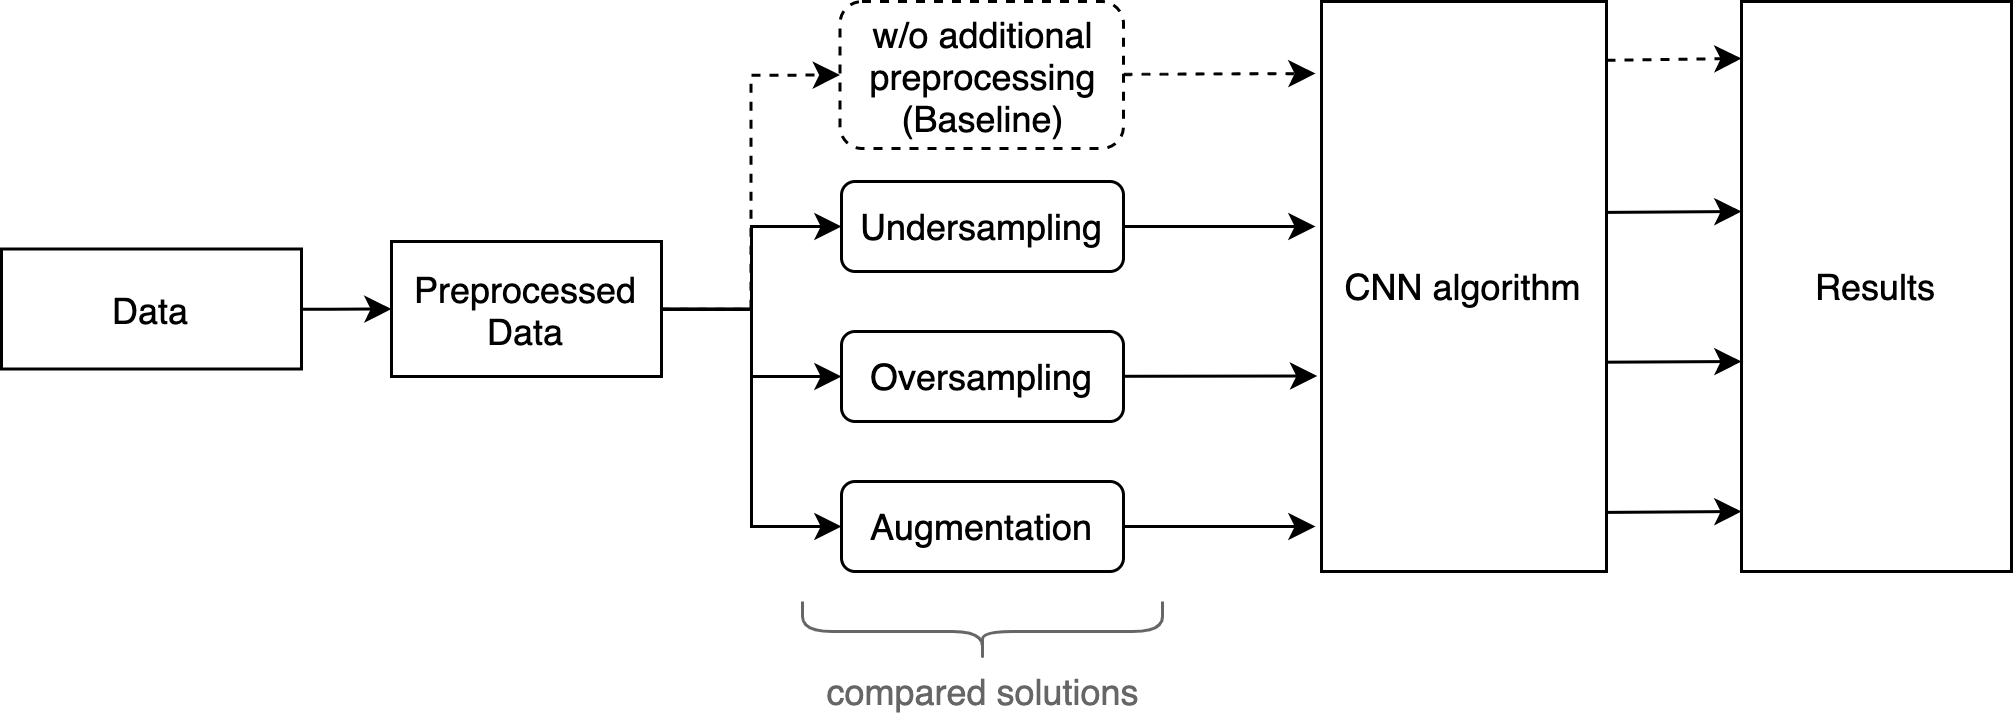
\includegraphics[width=\linewidth]{figures/planOfAttack.png}
  \caption{Way of Proceeding}
  \label{fig:plan}
\end{figure}

%% data exploration
\section{Data Set}
\subsection{Raw Data}
On Kaggle, a machine learning and data science community, users can provide datasets for other users. One such dataset is the “Chest X-Ray Images (Pneumonia)” dataset provided by the user Paul Mooney \cite{mooney2018}.  This dataset contains 5,863 x-ray images in JPEG format which are either classified as “normal”, having no pneumonia, “bacterial pneumonia” and “viral pneumonia”. Figure \ref{fig:kagglePneumonia} shows three exemplary images from the dataset which was provided by the creator of the dataset: 

\begin{figure}[h]
  \centering
  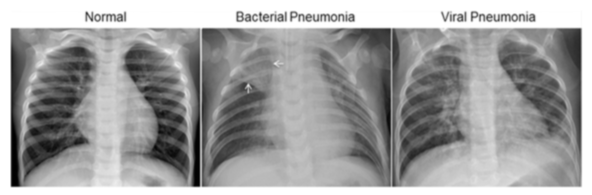
\includegraphics[width=\linewidth]{figures/Kaggle_x_ray_example.png}
  \caption{Exemplary x-ray images from the data set} 
  \label{fig:kagglePneumonia}
\end{figure}

The dataset is split into the train, validation and test set. The images were classified by two expert physicians and cleaned for low quality or unreadable scans. Additionally, the test set was verified by a third expert.
\subsection{Data Exploration}
The dataset contains 5,863 images in total. The dataset was split in a training, validation and test set from the provider of the dataset. Of those 5,863 images, 5,216 are in the training set, 16 in the validation set and 624 in the test set. Why the provider of the dataset has chosen this particular data split is unclear. 

\begin{figure}[h]
  \centering
  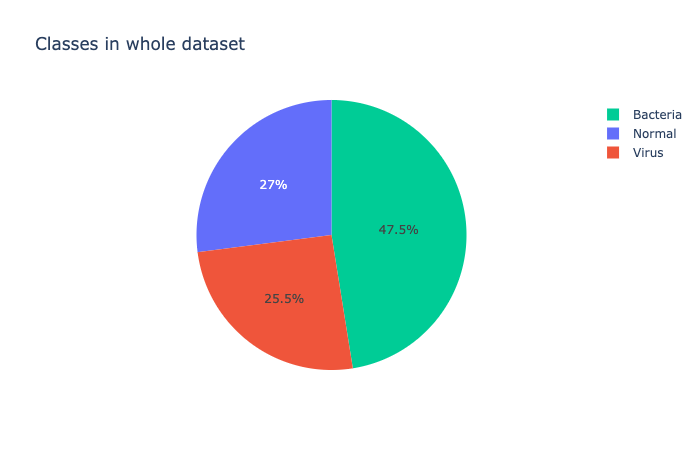
\includegraphics[width=\linewidth]{figures/pieChartClasses.png}
  \caption{Pie Chart of Classes in Data Set}
  \label{fig:data}
\end{figure}

Not only is the validation set with 16 images extremely small, which will likely cause problems, but the dataset’s classes are imbalanced as can be seen in figure \ref{fig:data}. 47.5\% of all classes in the dataset are a bacterial pneumonia infection, 25.5\% are labeled as a viral infection and 27\% have no condition. 

%% CNN
\section{Deep Learning Algorithm}
\subsection{Convolutional Neural Networks}
%% Why Convolutional Neural Networks (and not Naive Bayes)
Since our project deals with image classification, a deep learning algorithm was chosen, namely convolutional neural networks (CNN) as it is the state-of-the-art approach.\cite{szegedy2015going} Consequently, there are extensive libraries to utilize in this matter. In this research, the Keras library is used for the CNN in this paper.\\
A CNN takes raw image data as an input in the form of a multidimensional array. Each pixel represents a feature, possibly in several channels as it is a colored image (i.e. RGB) or a single channel as it is a grayscale image. Eventually, through training neurons by adapting weights and biases as an ordinary neural network does, class scores are received as an output. For a deeper understanding of the subject, see \cite{bloem2020deeplearning1}, \cite{karpathy2016convolutional}, on which our baseline code is based on. However, we included several conceptual changes as described later in this chapter.

\begin{figure}[h]
  \centering
  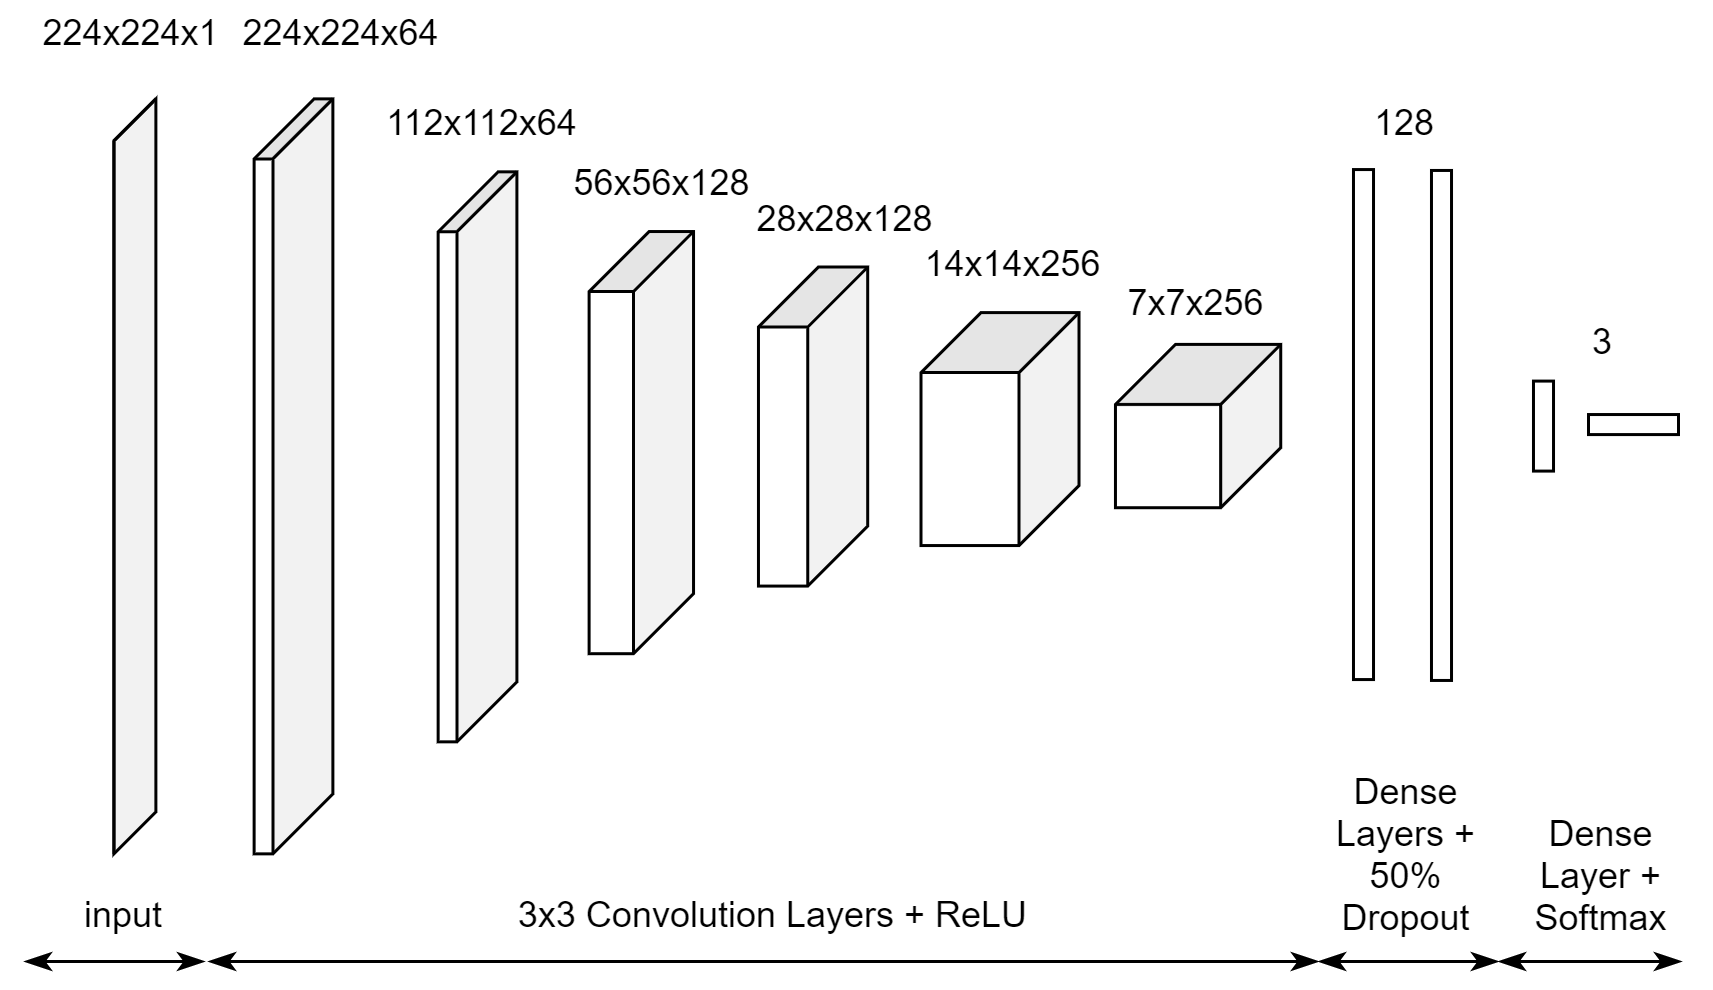
\includegraphics[width=\linewidth]{figures/cnn.png}
  \caption{schematic of the CNN used in this research}
\end{figure}

\subsection{Pre-Preprocessing}
%% Pre-Preprocessing: greyscale + Standardizing the images (224x224)
Our research discusses the influence of pre-processing measures to reduce class imbalance. To be able to compare the impact of those measures we define our raw data set not as given in Kaggle, but after some preceding preprocessing.\\
First, we change the classes from "Normal" and "Pneumonia" to "Normal", "Bacteria" and "Virus". \\
Second, we leave the separated test data as it is. We include the given validation set, as we consider it too small, to our training set, just to conduct a random 30\% split to separate the validation from the training data. According to \cite{bloem2020deeplearning1} it is considered best to have a validation set roughly the same size of the training set. Eventually, we choose a 30\% split, so that the now fixed validation set is also in a proper relation to even a smaller data set like the one prepared for undersampling.\\
Moreover, we standardize the data with $resize$ to 224x224 pixel images, which is a common number for input data \cite{karpathy2016convolutional}. Despite missing expertise in the field of pneumonia, we feel that this rescale preserves enough information while minimizing required memory and therefore speeding up the model fitting.\\
To slim down our model even further by reducing the channels from RGB to grayscale. The x-rays are already black and white, so this information is definitely abundant.\\
Eventually, this data will undergo additional preprocessing for further assessment dealing with class imbalance, which is described corresponding chapters on dealing with class imbalance.\\

\subsection{Model Fitting}
%% Strides vs Maxpooling
Based on the work of Springenberg et al. we refrain from pooling our data after every second convolution (with a single stride) as suggested in \cite{bloem2020deeplearning1}, \cite{karpathy2016convolutional}. As stated in \cite{springenberg2014striving}, it is sufficient to double the stride without losing any accuracy. This approach is called the all-convolutional net. For a concise introduction, see \cite{becker2018}.\\
%% Convolution
We stack twelve convolutional hidden layers in total including a ReLU activation layer after each convolution resulting in decreasing the image size while increasing the kernel size after every second convolution. Adding any more convolutional layers to our model have been proven counter-productive.\\ 
%% Flatten + Dropout
After the convolution layers, we flatten our data twice with dense layers. However, we avoid fully connected layers by dropping out 50\% of the data \cite{hinton2012improving} to counter overfitting \cite{srivastava2014dropout}. \\
% Regularization
However, in figure \ref{fig:cnn_opt_a} we also see that Dropout is not enough to deal with overfitting. After 12 epochs the loss function in the validation set increases again after dropping initially. That is why we also added L2-regularization for further improvement, this drastically improves the overfitting behaviour. Comparing the regularization arguments, we choose r=0.1, as it shows the best results with our model (figure \ref{fig:cnn_opt_c}). \\
%% Batchsize + Epochs
As suggested in \cite{bloem2020deeplearning1} we train our model in mini batches to utilize both advantages of stochastic gradient descent with its ability to escape local minima and full batch with increased parallelism, while also reducing the variance with bigger batches. The batch size is restricted by the GPU memory provided by Google Colaboratory, which we used in our project. As seen in figure \ref{fig:cnn_opt_b}, increasing batch size also has a positive influence on reducing overfitting. Therefore, we choose a batch size of 128, which also marks the upper boundary recommended in \cite{bloem2020deeplearning1}.\\
In total, we train the neural network in 30 epochs since our target functions have plateaued off.
\begin{figure}[!ht]
  %\begin{minipage}{0.5\linewidth}
    \centering
    \subfloat[influence regularization]{\label{fig:cnn_opt_a}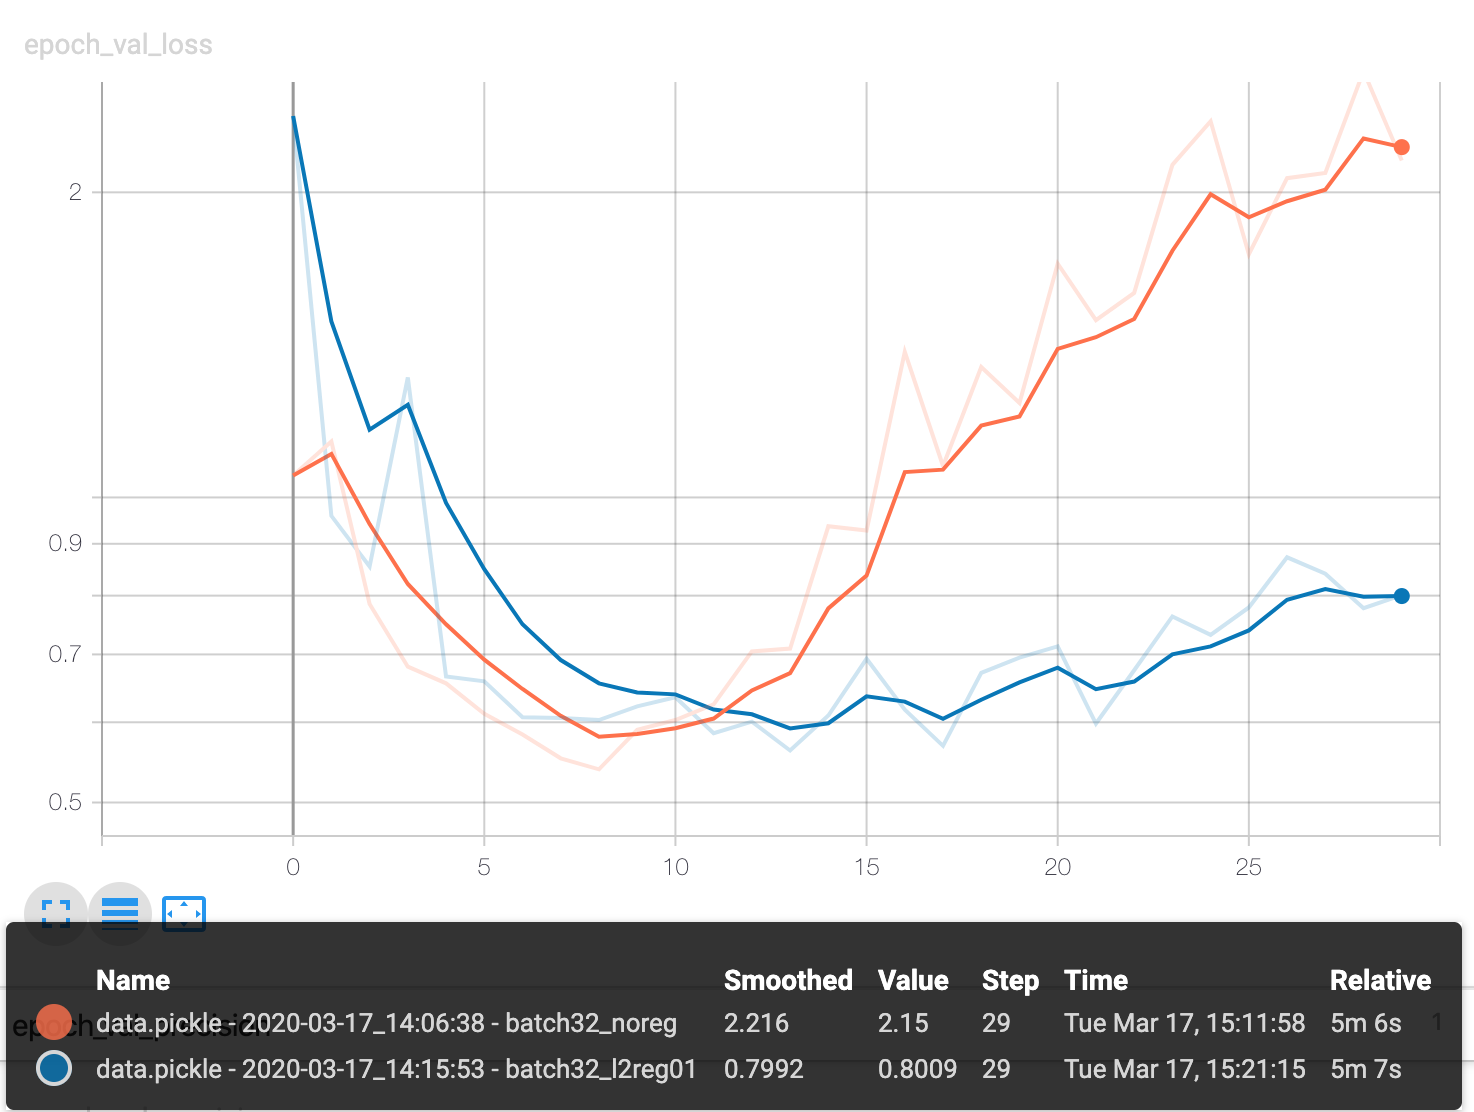
\includegraphics[width=0.89\linewidth]{figures/noregCompare.png}}
    \par\medskip
  %\end{minipage}%
  %\begin{minipage}{0.5\linewidth}
    \centering
    \subfloat[influence batchsize]{\label{fig:cnn_opt_b}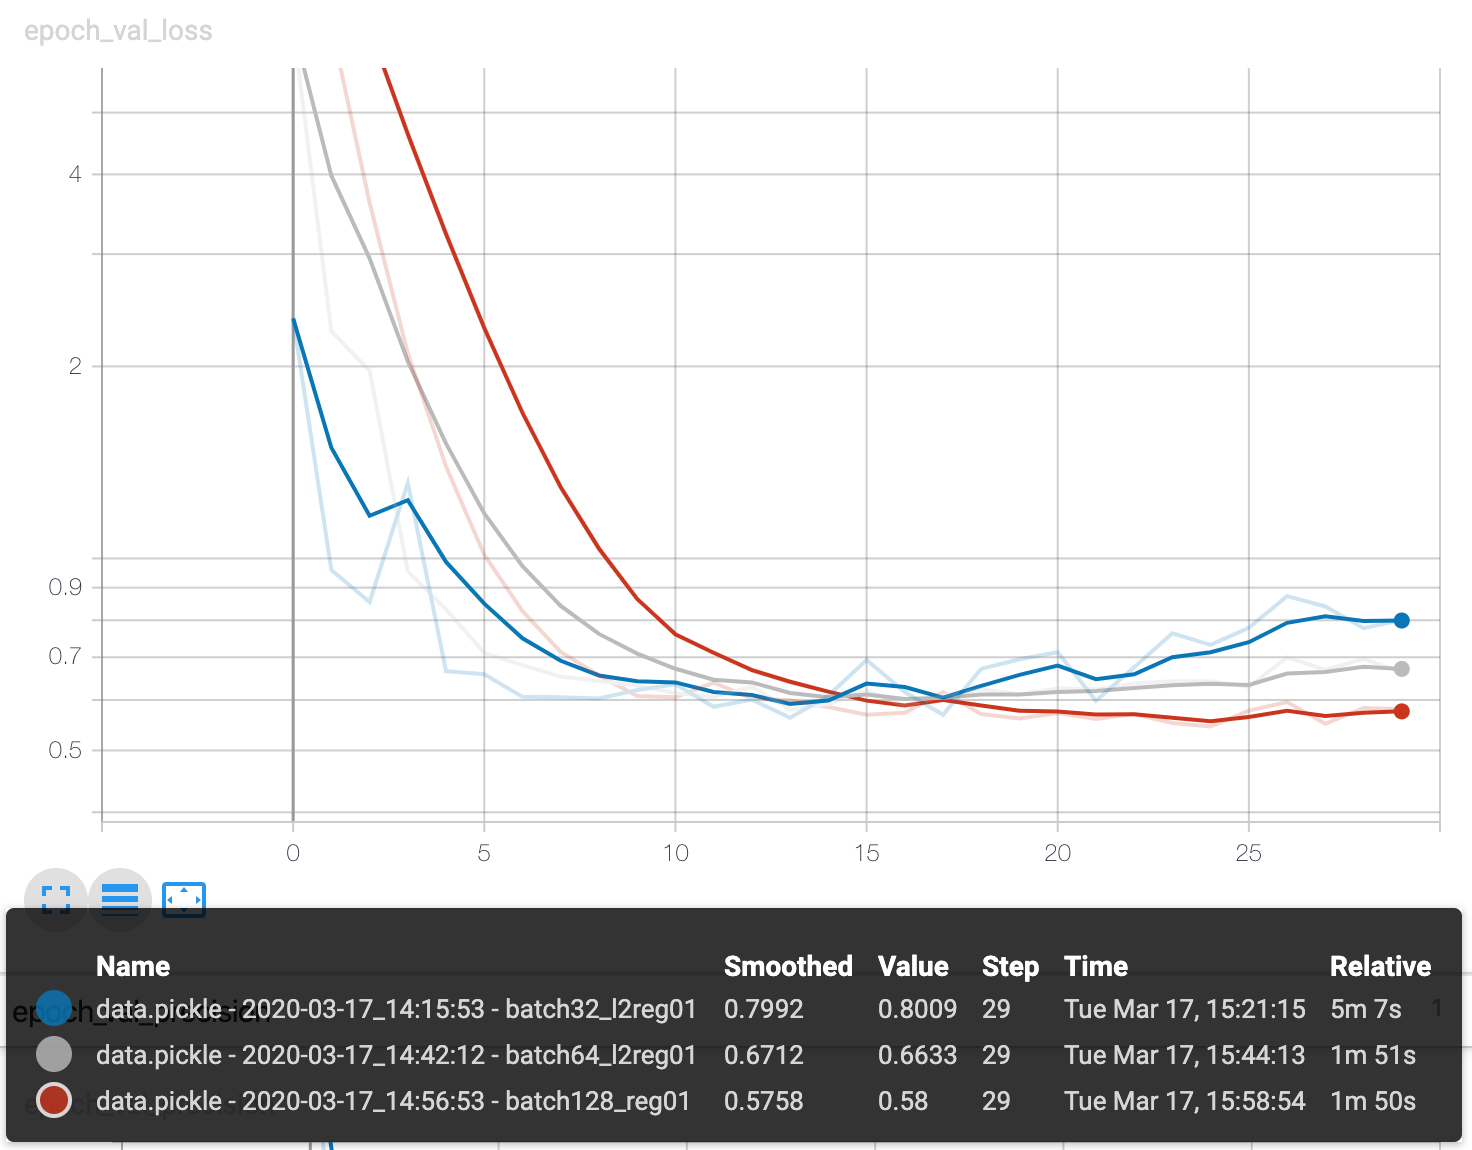
\includegraphics[width=0.89\linewidth]{figures/batchCompare.png}}
    \par\medskip
  %\end{minipage}\par\medskip
    \centering
     \subfloat[influence regularization parameter]{\label{fig:cnn_opt_c}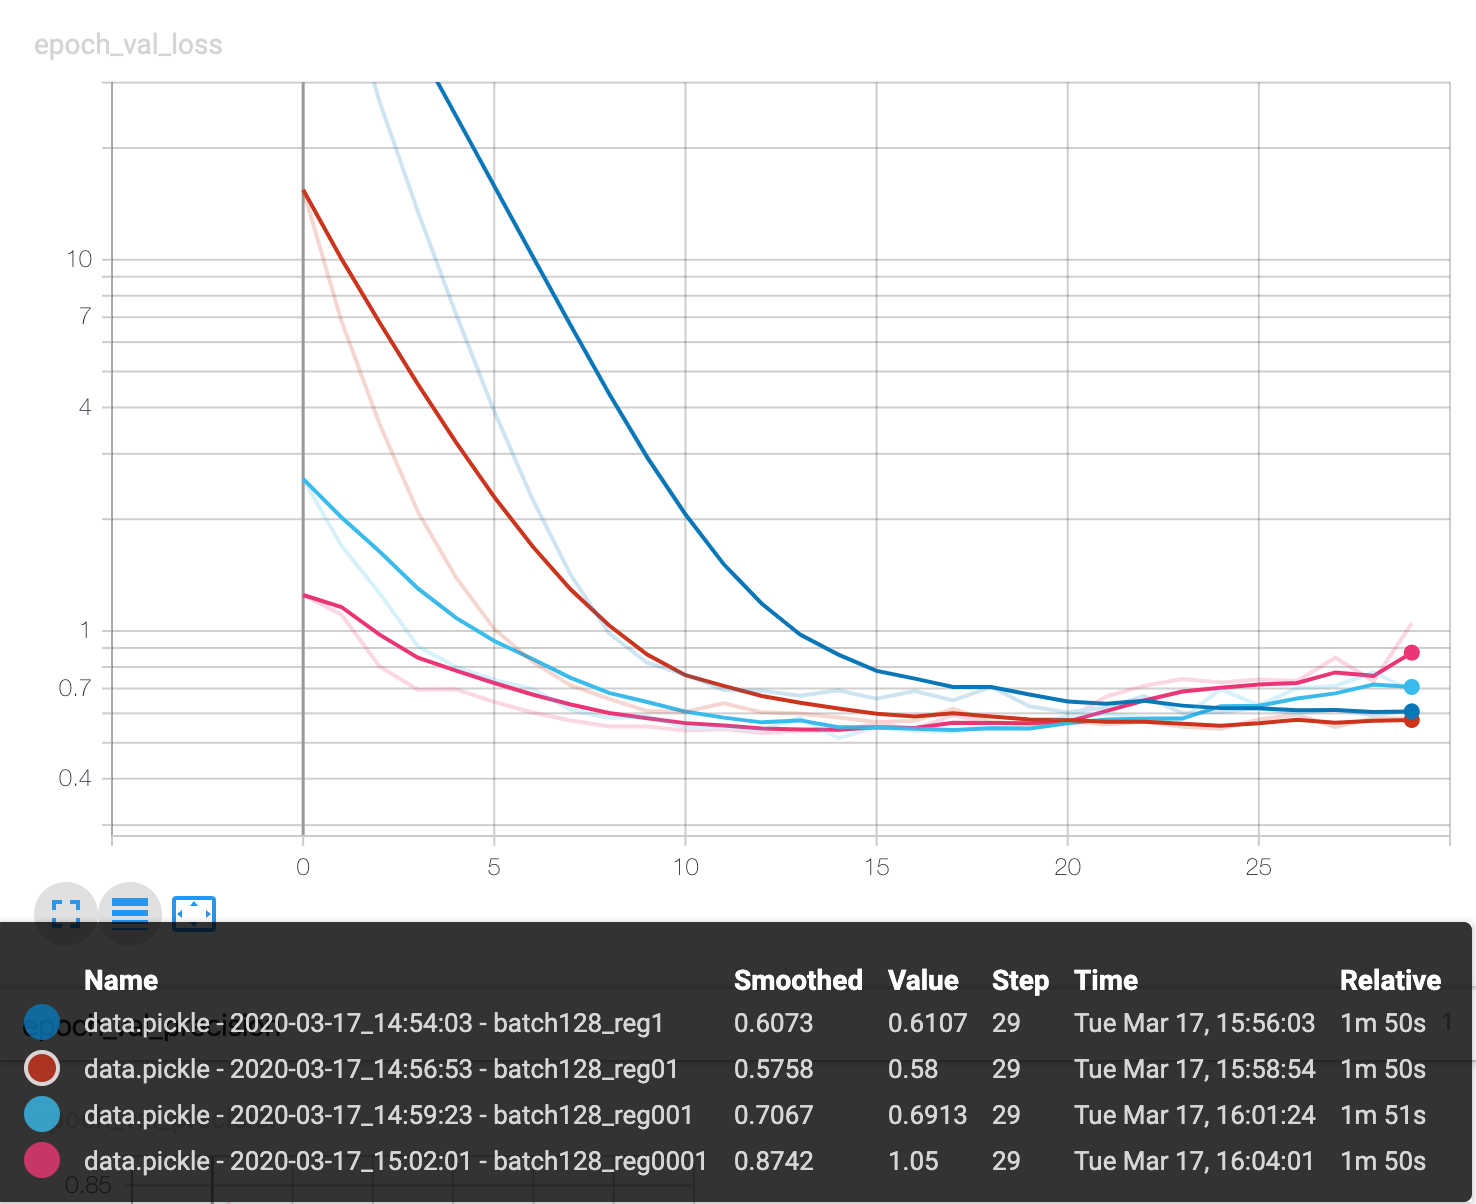
\includegraphics[width=0.89\linewidth]{figures/regCompare.png}}
    \par\medskip
  \caption{Optimizing the CNN algorithm}
  \label{fig:opt}
\end{figure}

%% baseline
\section{Baseline}
\subsection{Assessment Method}
All results are assessed by the precision metric in combination with the recall metric. The higher both metrics, the better.  However, recall is given more weight. Precision returns a proportion of how many images were classified correctly, e.g. of all images identified as class X, how many actually have class X? Recall returns a proportion of how many images have been identified as relevant which are "actually" relevant, e.g. of all images classified as Y, how many were detected as class Y correctly? The recall metric is especially important for this particular classification task as it is used for medical diagnosis.\cite{powers2011evaluation} If the recall metric is low, then images that are classified as (having) "pneumonia" are not detected as (having) "pneumonia". This "false negative" would be a disaster in a real-life scenario. The patient is diagnosed as having no pneumonia although he or she has pneumonia. In other words, the pneumonia would remain undetected. The worst case scenario of low precision would be that patients are diagnosed with having pneumonia, although they don't have pneumonia. This would be a "false positive". In a real life scenario this would likely lead to a more in depth investigation which would revoke the former diagnosis as a "false-alarm" which eventually does not harm the patient.

% As described in the baseline chapter, the goal is to achieve high precision in combination with a high recall score. The recall score is given more weight since the number of false negatives should be as low as possible. All methods will be assessed with these metrics on the validation set.



The equations are defined as following:
\begin{equation}
Precision = \frac{TP}{TP +  FP}
\end{equation}
\begin{equation}
Recall = \frac{TP}{TP +  FN}
\end{equation}
Where TP is defined as true positives, FP as false positive and FN as false negative.\\
Suppose the data set contains 100 x-ray images in total. Of these, 40 images are classified as "normal", therefore negative, while 60 are classified as (having) "pneumonia", therefore positive.\\
On the one hand, the CNN classifies 68 images as positive of which 57 classifications are correct (true positive) while 11 were identified positive although they were negative (false positive).\\ 
On the other hand, the CNN classifies 32 images as negative of which 29 classifications are correct (true negative) while 3 were identified negative although they were positive (false negative).\\
Therefore in this example the precision would be $\frac{57}{68}$ and the recall would be $\frac{57}{60}$.


%This gives the following confusion matrix: \\
\begin{table}[h]
    \centering
    \begin{tabular}{l|l|c|c|c}
\multicolumn{2}{c}{}&\multicolumn{2}{c}{True diagnosis}&\\
\cline{3-4}
\multicolumn{2}{c|}{}&Positive&Negative&\multicolumn{1}{c}{Total}\\
\cline{2-4}
\multirow{2}{*}{Screening test}& Positive & \cellcolor{green}$57$ & \cellcolor{red}$11$ & $68$\\
\cline{2-4}
& Negative & \cellcolor{red}$3$ & \cellcolor{green}$29$ & $32$\\
\cline{2-4}
\multicolumn{1}{c}{} & \multicolumn{1}{c}{Total} & \multicolumn{1}{c}{$60$} & \multicolumn{    1}{c}{$40$} & \multicolumn{1}{c}{$100$}\\
\end{tabular}
    \caption{Confusion Matrix}
    \label{tab:my_label}
\end{table}

\subsection{Results}
Using the developed CNN on the data set without any further pre-processing to deal with class imbalance yields the following results on the test set. The results will serve as the baseline for the solutions discussed in this paper: \\
\begin{equation}
Precision = 0.7087
\end{equation}
\begin{equation}
Recall = 0.7019
\end{equation}
\\
For comparisons of different methods in the upcoming chapters a "training baseline" is introduced. Training baseline refers to a baseline whose results are evaluated on the validation set instead of the test set. This ensures that the test set will not be used until the final evaluation and prevent multiple testing on the test set.


%% undersampling
\section{Undersampling}
\subsection{Undersampling Data Set}
Undersampling is a technique to deal with class imbalance, as introduced in \cite{bloem2020methology1}. This simple approach reduces class imbalance by excluding instances from the majority class. The majority class is identified and randomly chosen instances of majority class are excluded to match the number of instances of the minority class. This is done recursively till all classes have an equal distribution. The resulting dataset is visualized in figure \ref{fig:undersampling_class_distribution}.

% on the left before, on the right after
\begin{figure}[h]
    \centering
    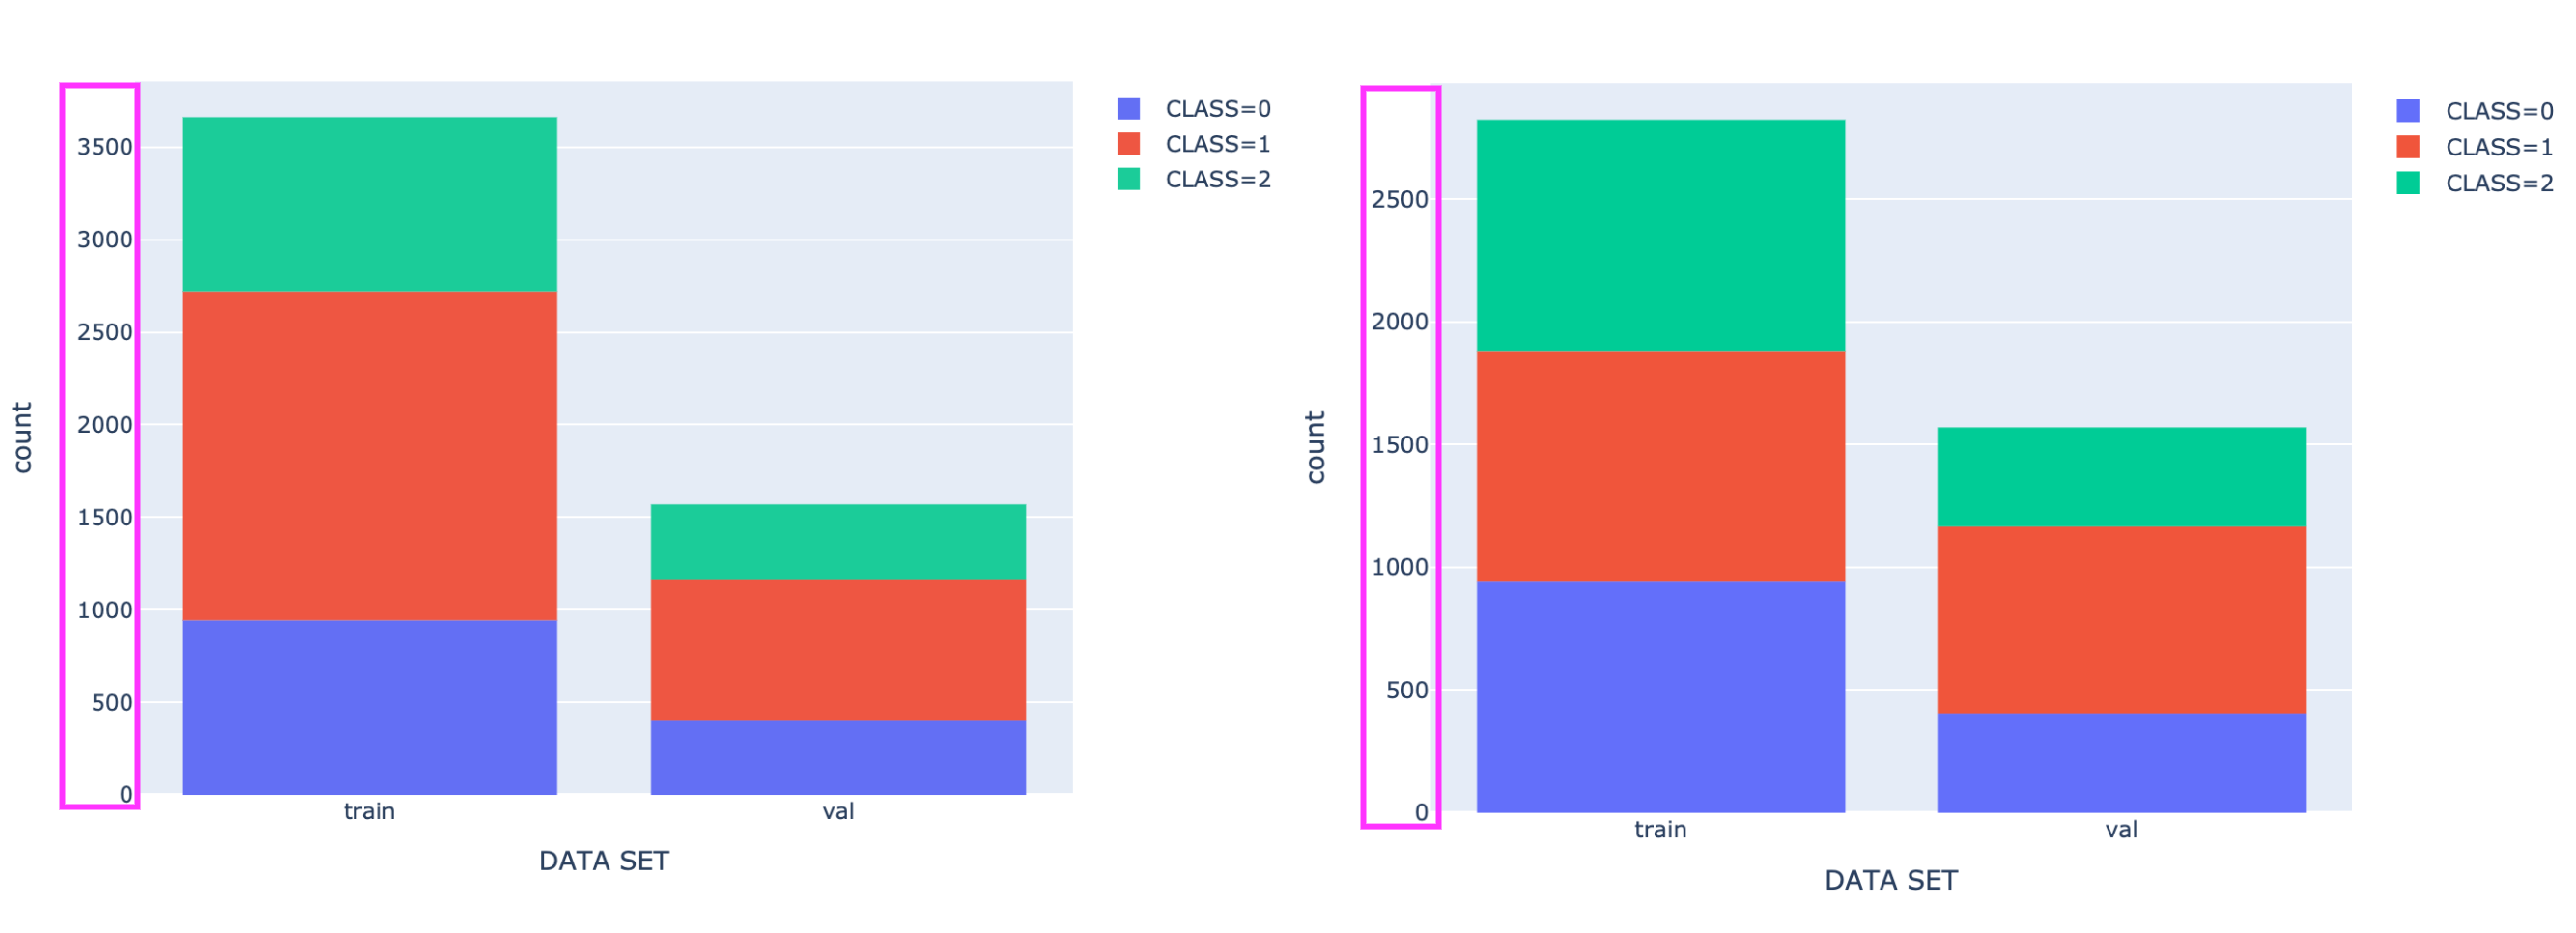
\includegraphics[width=\linewidth]{figures/undersampling/distribution_classes_before_after.png}
    \caption{Class distribution after undersampling. On the left before, on the right after. Note that the y-axis is scaled to the biggest dataset. Therefore, before and after are not shown on the same scale}
    \label{fig:undersampling_class_distribution}
\end{figure}

\subsection{Results on Validation Set} 
The CNN was trained three times with the undersampled data-set. The results, as can be seen in figure \ref{fig:under_val}, show no significant performance difference in both precision and recall compared to the baseline. The precision is in between a range of 0.80 to 0.82 in the baseline and training using the undersampled data-set with one outlying result which yields a result of 0.83. Both recall results are also in the same range from 0.78 to 0.80 except for the one outlying result which achieves a result of 0.82. 

\begin{figure}[!ht]
    \centering
    \subfloat[Precision]{\label{fig:under_val_a}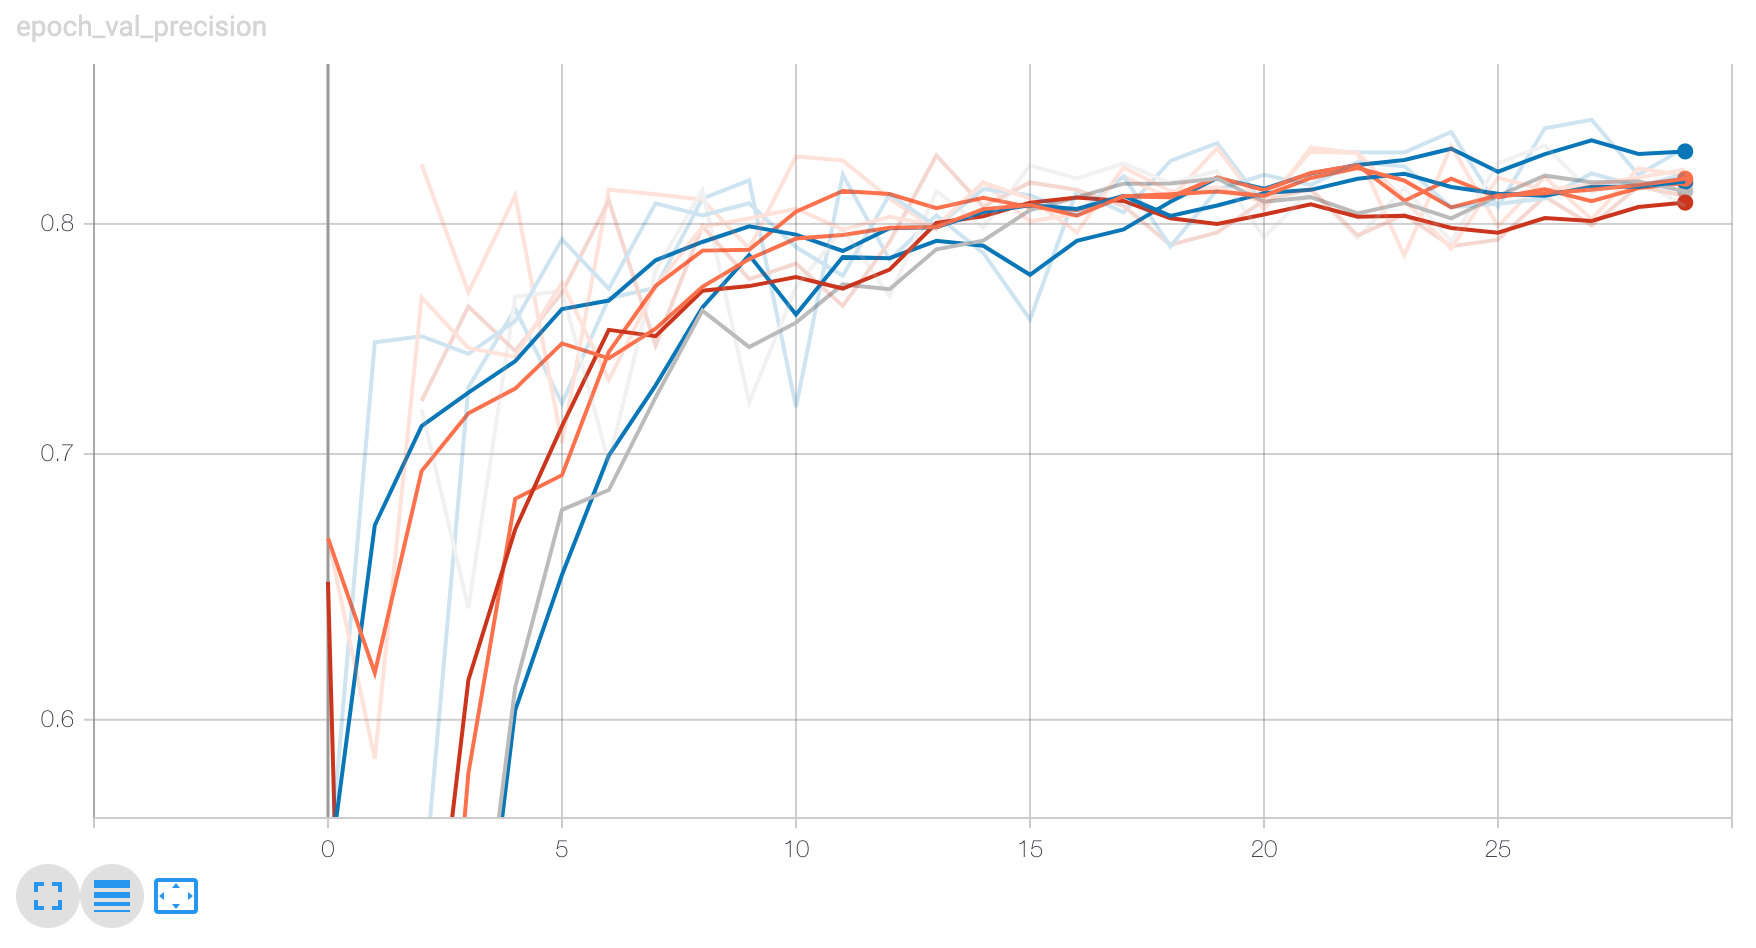
\includegraphics[width=0.89\linewidth]{figures/undersampling/val_precision.png}}
    \par\medskip
    \centering
    \subfloat[Recall]{\label{fig:under_val_b}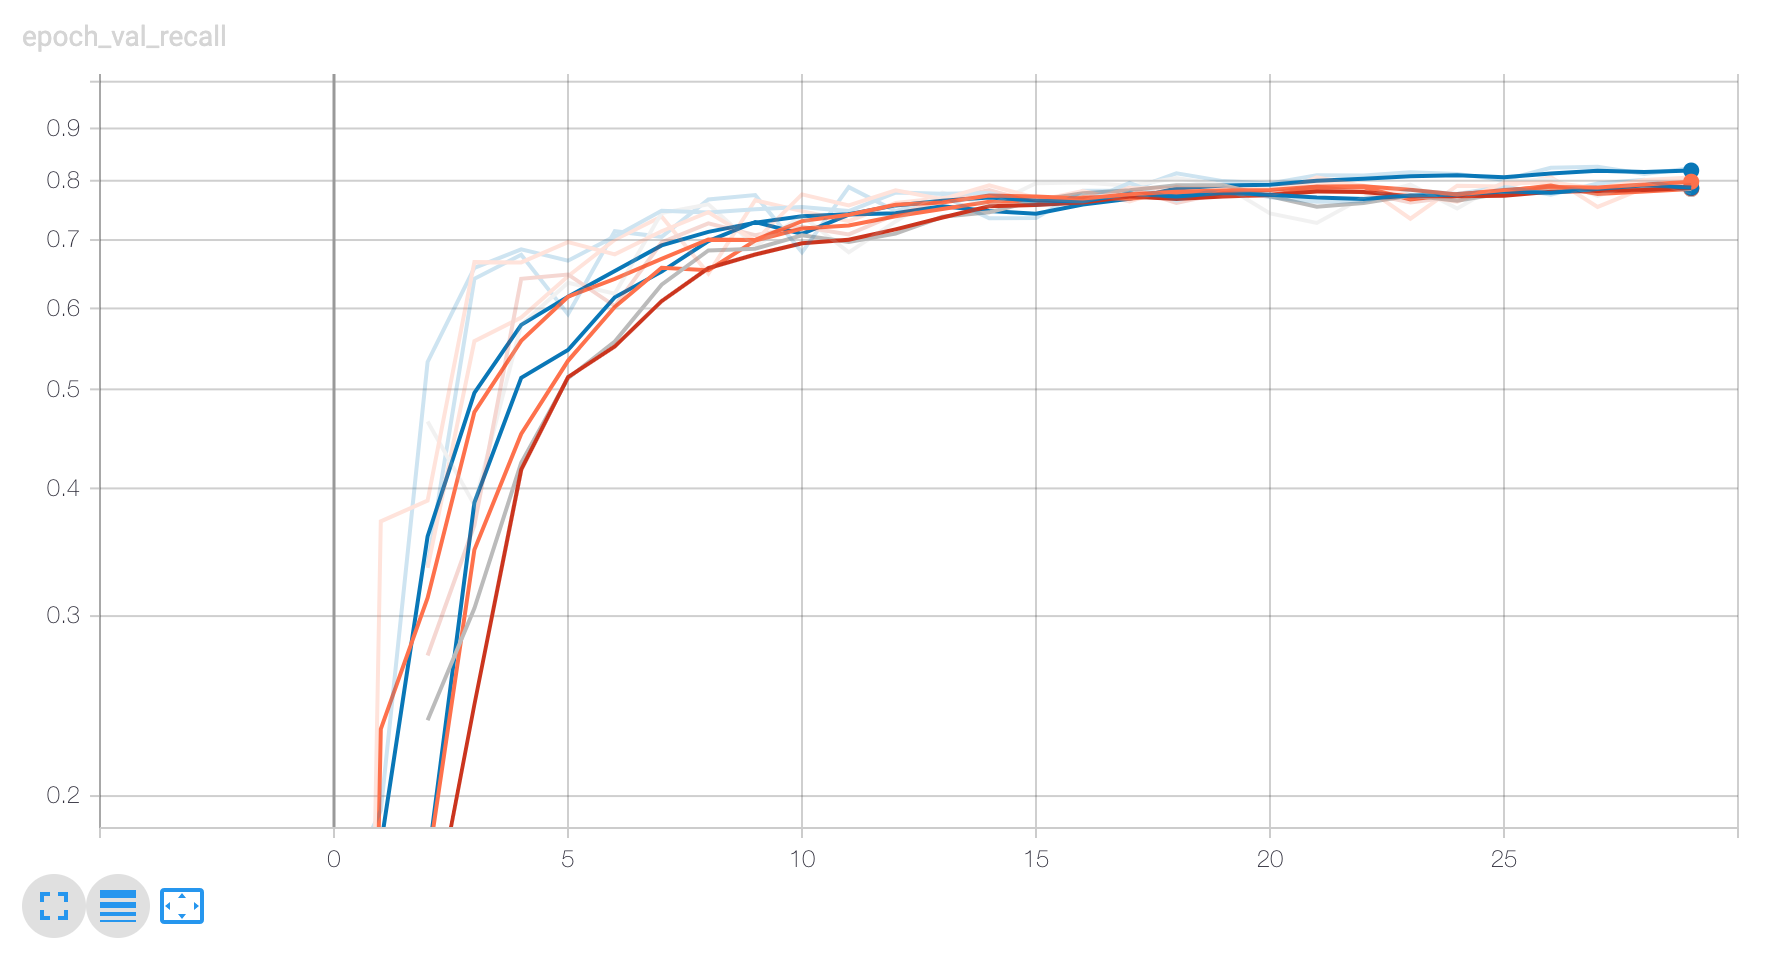
\includegraphics[width=0.89\linewidth]{figures/undersampling/val_recall.png}}
    \par\medskip
  \caption{Undersampling on Validation Set. The baseline and undersampling results are not clearly distinguishable which indicates no clear improvement or worsening.}
  \label{fig:under_val}
\end{figure}

\subsection{Results on Test Set}

\begin{equation}
Precision = 0.6770
\end{equation}
\begin{equation}
Recall = 0.6651
\end{equation}

No performance increase is achieved using undersampling. The differences on the validation set were thought to be due some randomness as the baseline also achieves different but very similar results. However, the results on the test set reveal that undersampling actually performs slightly worse than the baseline. \\
Reasons could be that we specifically made sure that the CNN is not overfitting. Undersampling lead to less training images which could have effected the overall results in a negative way. If the CNN would have overfitted with the original training set, we could have seen a positive result because the class imbalance, which would have likely lead to overfitting as can be seen in the oversampling chapter, would be neglected.   

%% oversampling
\section{Oversampling}

\subsection{Oversampling Data Set}
Oversampling is a technique to deal with class imbalance as introduced in \cite{bloem2020methology1}. This approach reduces class imbalance by duplicating some of the given images. The majority class is identified. The remaining classes are then "oversampled" to the same number of instances as the majority class. E.g. if the majority class has 2000 instances and the minority classes have 1300 and 1400 images, then the minority classes would get 700 and 600 additional "oversampled" instances (images). The resulting dataset is visualized in figure \ref{fig:oversampling_class_distribution}.

\begin{figure}[h]
    \centering
    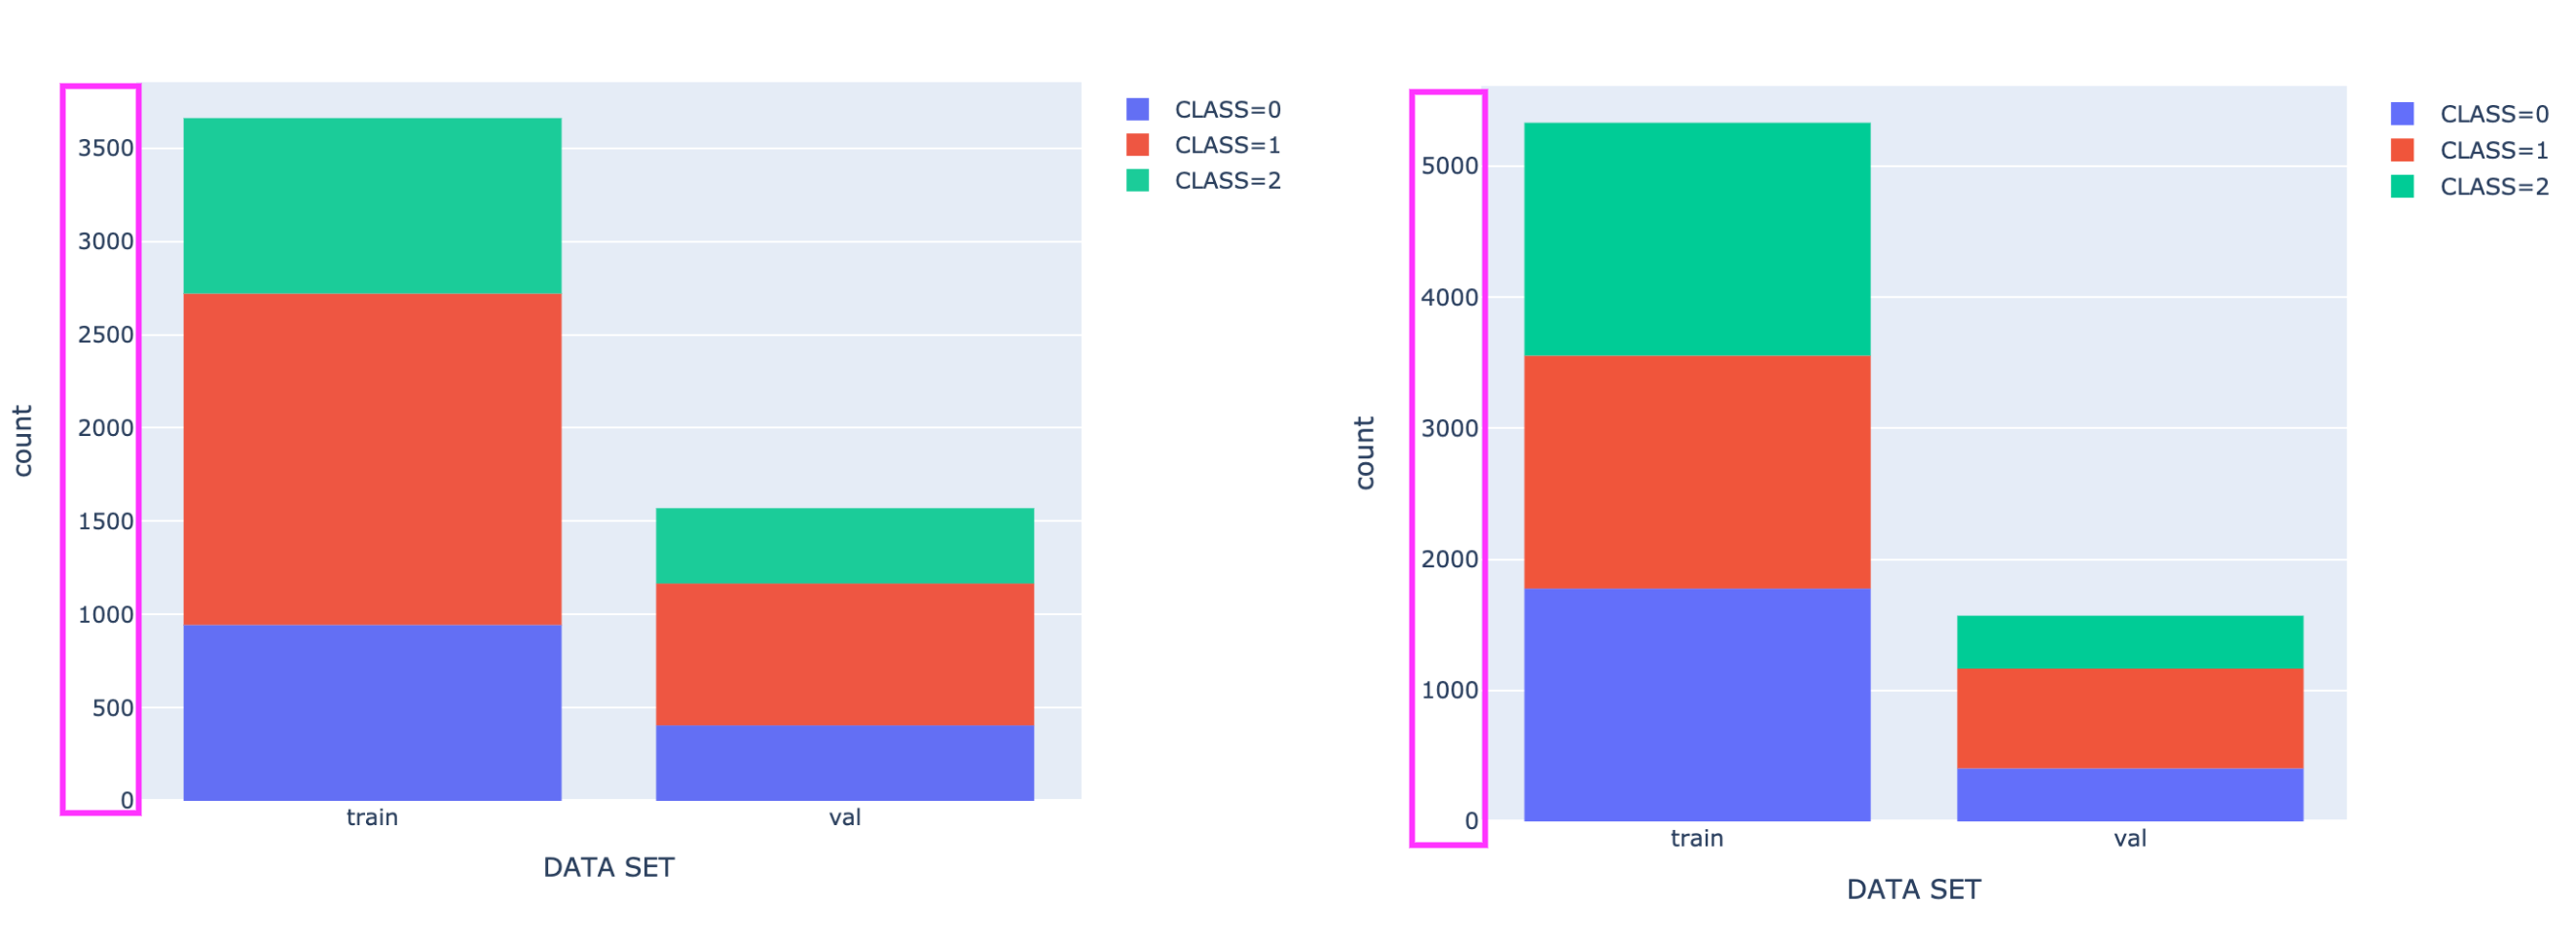
\includegraphics[width=\linewidth]{figures/oversampling/class_distribution_before_after.png}
    \caption{Class distribution after oversampling. On the left before, on the right after. Note that the y-axis is scaled to the biggest dataset. Therefore, before and after are not shown on the same scale}
    \label{fig:oversampling_class_distribution}
\end{figure}

\subsection{Results on Validation Set}
The CNN was trained three times with the oversampled data set. The results, as can be seen in the figures, show substantial worse performance in both precision and recall on the validation set compared to the baseline. While the precision on the validation set is in between a range of 0.80 to 0.82 in the baseline, the precision is only in a range of 0.27 to 0.28 using the oversampled dataset as can be seen in figure \ref{fig:over_val_a}. Likewise is the recall metric. The baselines results are in between a range of 0.78 to 0.80 while the usage of the oversampled dataset yields results in a range of 0.27 to 0.28 as can be seen in figure \ref{fig:over_val_b}.

\begin{figure}[!ht]
    \centering
    \subfloat[Precision]{\label{fig:over_val_a}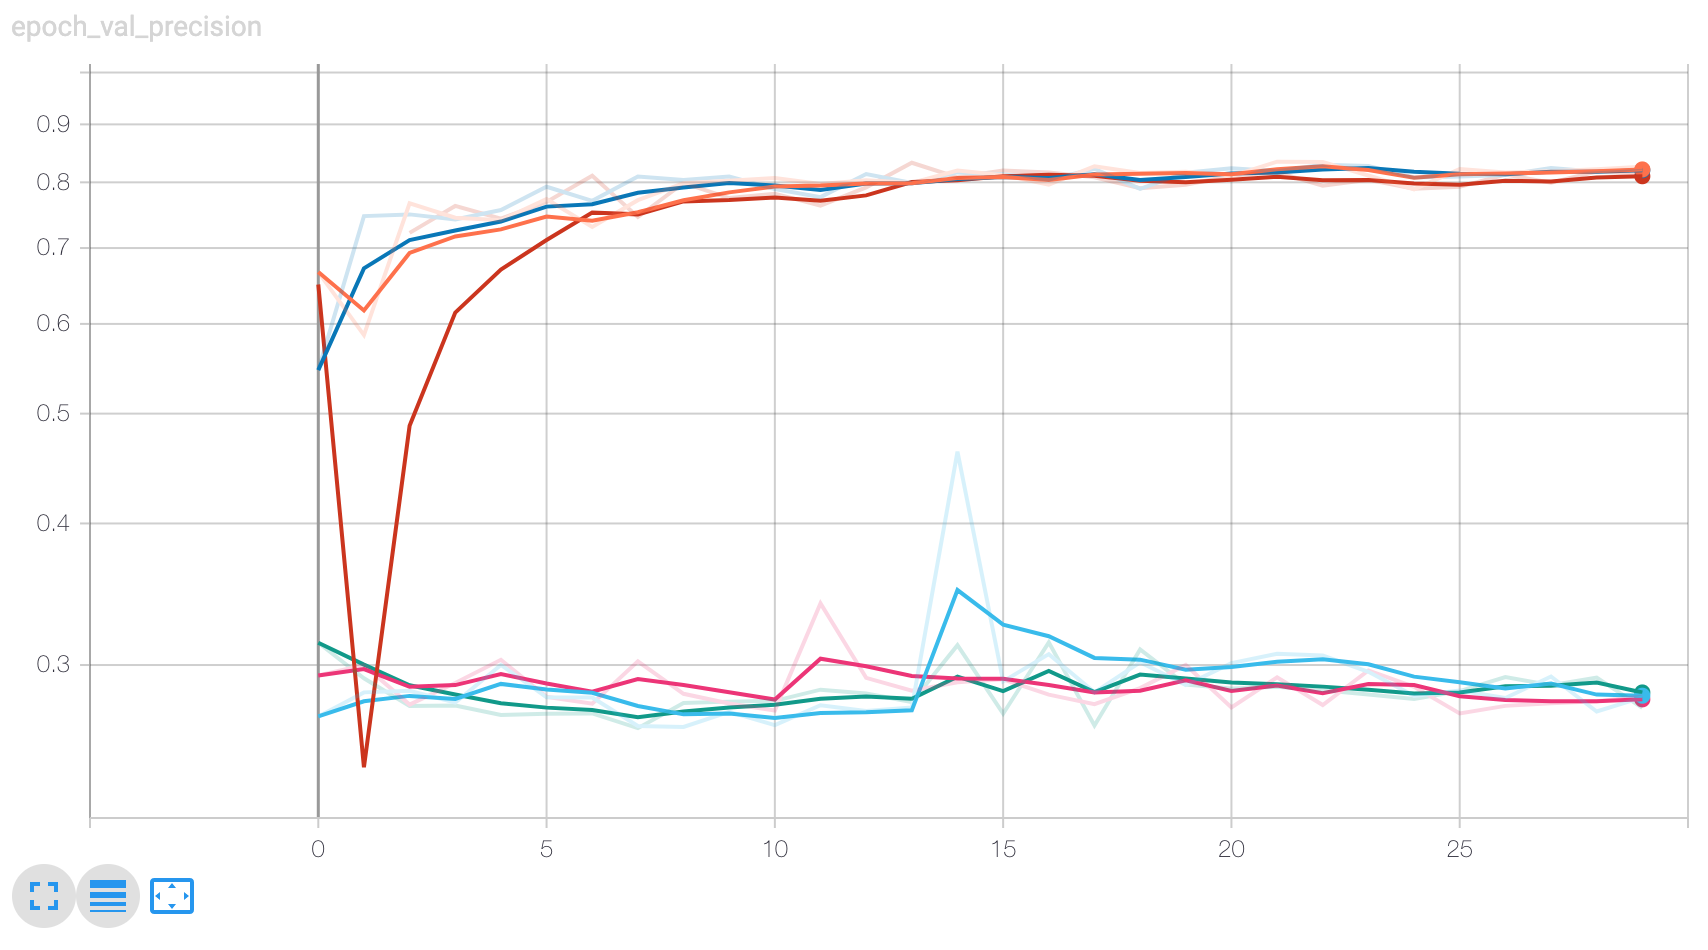
\includegraphics[width=0.89\linewidth]{figures/oversampling/val_precision.png}}
    \par\medskip
    \centering
    \subfloat[Recall]{\label{fig:over_val_b}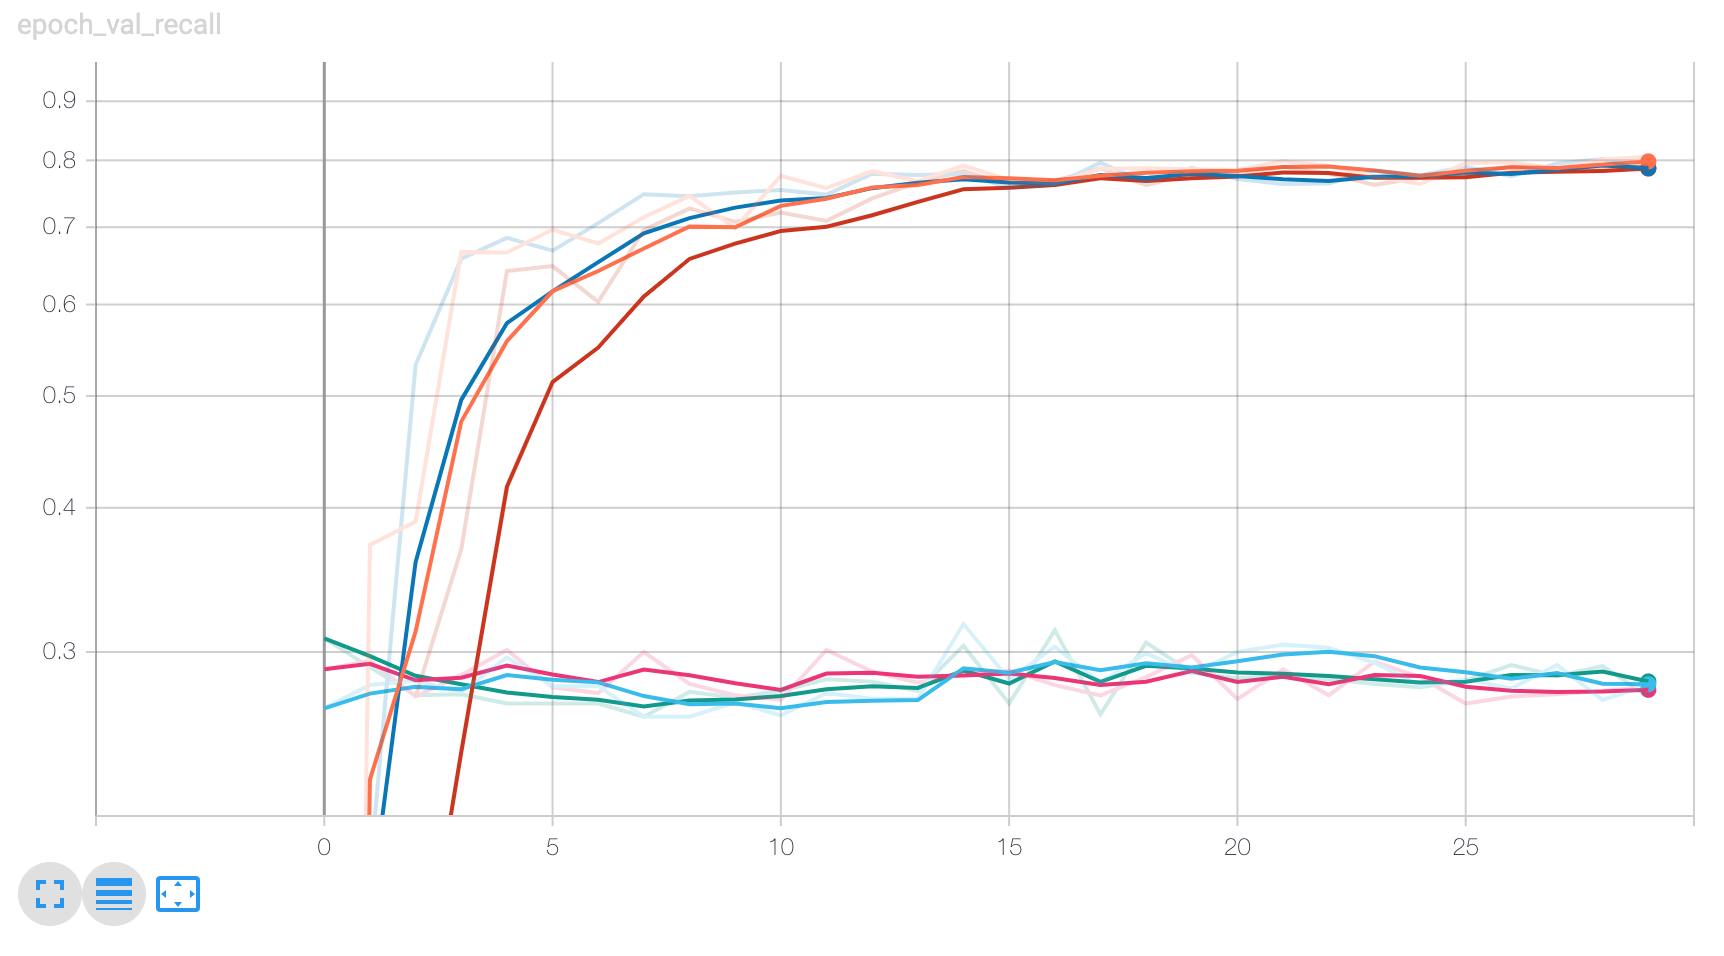
\includegraphics[width=0.89\linewidth]{figures/oversampling/val_recall.png}}
    \par\medskip
  \caption{Oversampling on Validation Set. The baselines are the three lines in the upper part of the graph. The results of oversampling are the three bottom lines. As can be seen, oversampling performs worse than the baseline.}
  \label{fig:over_val}
\end{figure}

Looking into the precision and recall results on the train set reveals that the CNN highly overfits when trained with the oversampled dataset. After already 10 batches both precision and recall above 0.995 which is near perfect when the CNN is trained with the oversampled data set as can be seen in figure \ref{fig:over_train}.
\begin{figure}[!ht]
    \centering
    \subfloat[Precision]{\label{fig:over_train_a}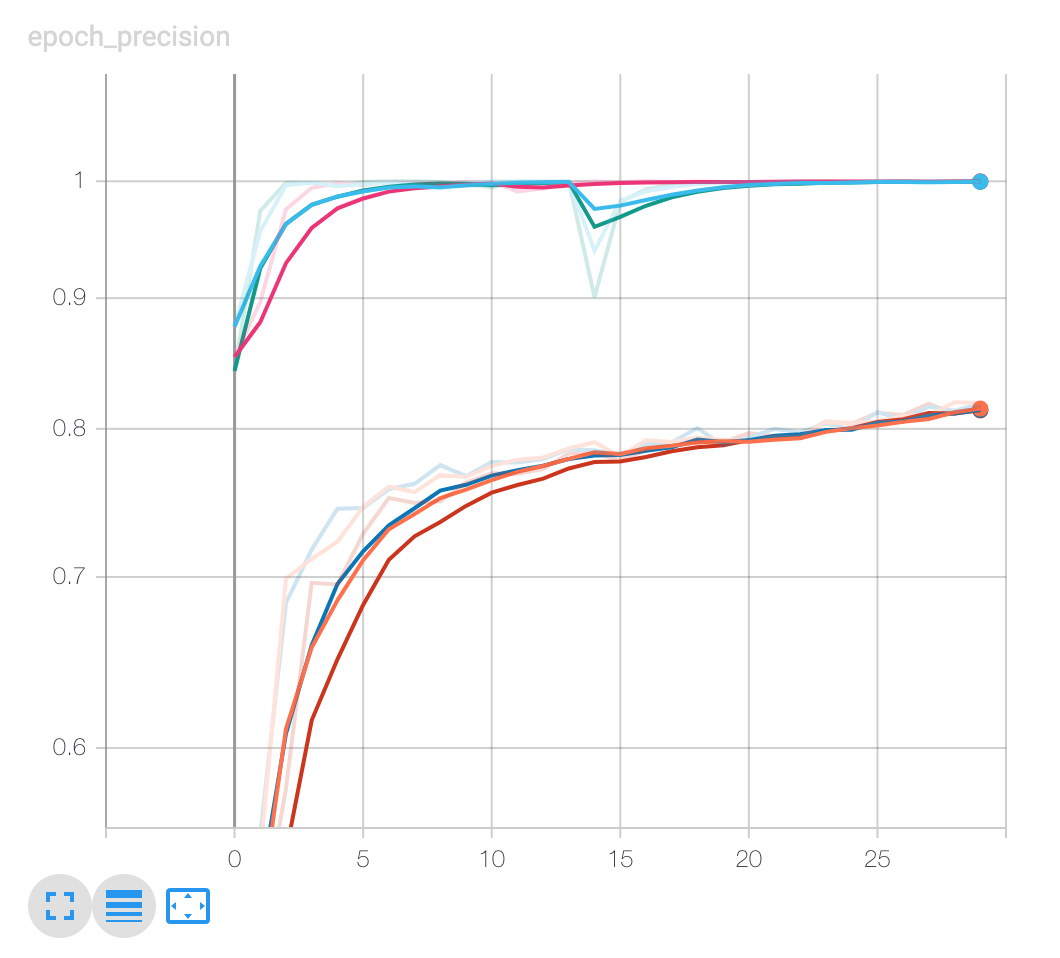
\includegraphics[width=0.89\linewidth]{figures/oversampling/train_precision.png}}
    \par\medskip
    \centering
    \subfloat[Recall]{\label{fig:over_train_b}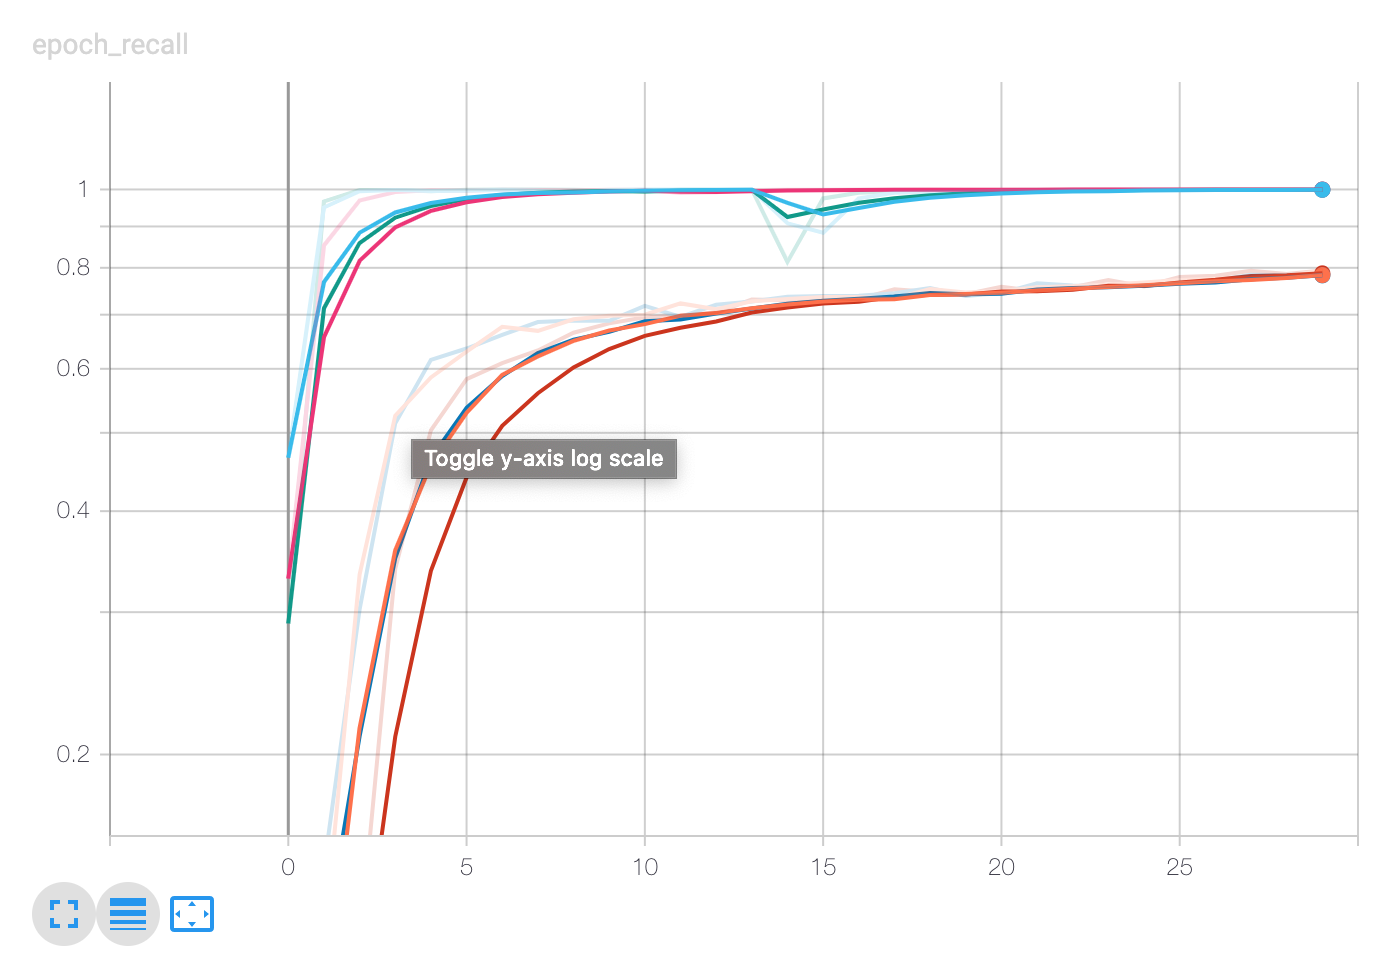
\includegraphics[width=0.89\linewidth]{figures/oversampling/train_recall.png}}
    \par\medskip  \caption{Oversampling on Training Set. The baselines are the three lines in the lower part of the graph. The results of oversampling are the three lines in the upper part of the graph. As can be seen, the oversampling results achieve near full precision and recall after a few number of batches. This implies high overfitting.}
  \label{fig:over_train}
\end{figure}

% RUN ON TEST SET

\subsection{Results on Test Set}

\begin{equation}
Precision = 0.3720
\end{equation}
\begin{equation}
Recall = 0.3702
\end{equation}

The results from on the validation set are replicated on the test set although the results on the test set are substantially higher, from around 0.27 in both metrics to around 0.37, but still way below the baseline. \\
The conclusion is drawn that oversampling in this setup leads to overfitting and therefore to worse performance. 


%% augmentation
\section{Data Augmentation}
\subsection{Data augmentation methods}
There are few different ways how to deal with class imbalance using augmentation \cite{bloem2020methology1}. Horizontal and vertical shifting, zooming, tilting and vertical flipping (mirroring) is used to augment the underrepresented classes. This is achieved with the "ImageDataGenerator" function from the Keras framework \cite{imagepreprocessing-kerasdocumentation}. \\


\subsection{Method}
The data is augmented using the "ImageDataGenerator" function from Keras for each class. ImageDataGenerator has multiple parameters which influence the augmentation of images. Width-shift range, height-shift range, rotation-range, zoom-range and vertical-flip are used. Height-shift and width-shift range "shift" the images in a given range of for example 10 pixels in height, width or combined. Rotation-range "rotates" an image by a certain degree given in the set range. Zoom-range "zooms" an image by a given percentage. Vertical-flip "mirrors" the image.\\
The amount of the to be generated images is determined by a function that detects the most occurring class, counts the images available for this class and creates augmented images for the underrepresented classes to match the amount of images of the most occurred class. After the creation of the augmented images, the images are merged with a copy of the original training set. This results in a new data set without class imbalance with variations of the augmented images set in the "ImageDataGenerator" function.\\
Each parameter was tested individually with different values and in every possible combination with the other parameters. This resulted in 164 different combinations. Due to limited hard drive capacity, cloud storage capacity (the augmented data was 55GB big) and training time, more combinations could not be tested. \\
The width- and height-shift were both tested with a shift range of 0, 5 and 10.\\
The zoom-range was tested with a percentage of 0, 10 and 20. \\
The rotation-range was tested with 0,10 and 20 degrees. \\
Vertical-flip was tested with the values 0 for off and 1 for on.\\

\subsection{Initial results on validation set}
Initially, the train and validation set was created each time the CNN was trained instead of splitting the dataset (excluding the test set) into the train and validation set once. This meant that augmented data was in both the training and validation set.\\
This lead to the phenomena that the results would not differ from the training baseline when taking into consideration some randomness. Even when shifting the images by up to 224 pixels (the whole width or height) the results would not differ. Figure \ref{fig:shift_img} is an example of such an extreme augmentation but not the most extreme, some pictures were just black.
\begin{figure}[h]
    \centering
    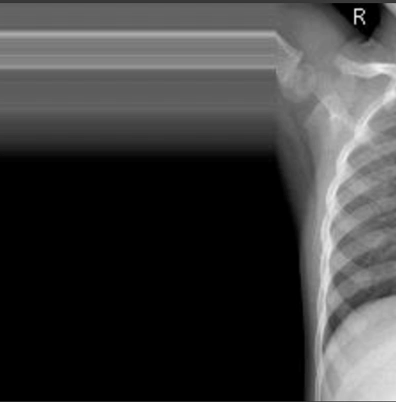
\includegraphics[width=0.4\linewidth]{figures/augmentation/faulty_image_example.png} 
    \caption{Notable Shifting of Image}
    \label{fig:shift_img}
\end{figure}
This should not yield the same results as the training baseline, but initially it did. The problem was likely the split at the beginning of each training. The "faulty" augmented data was present in both the train and validation set. Our design decision to create a train and validation set each for each training introduced errors to the validation set which would have likely resulted in devastating results on the test set.

\subsection{Results on Validation Set} 
To correct the introduction of faulty data into the validation set, the train and validation set split was changed to happen only once.\\
Surprisingly, even this corrected method did not show substantial differences from the training baseline, which would allow for a confident conclusion that this data augmentation method does indeed result in better results and the different results are not just due to some randomness. \\
All 164 results yield results in both precision and recall in a similar range as the training baseline. Which can be seen in figure \ref{fig:augm_val}.

\begin{figure}[!ht]
    \centering
    \subfloat[Precision]{\label{fig:augm_val_a}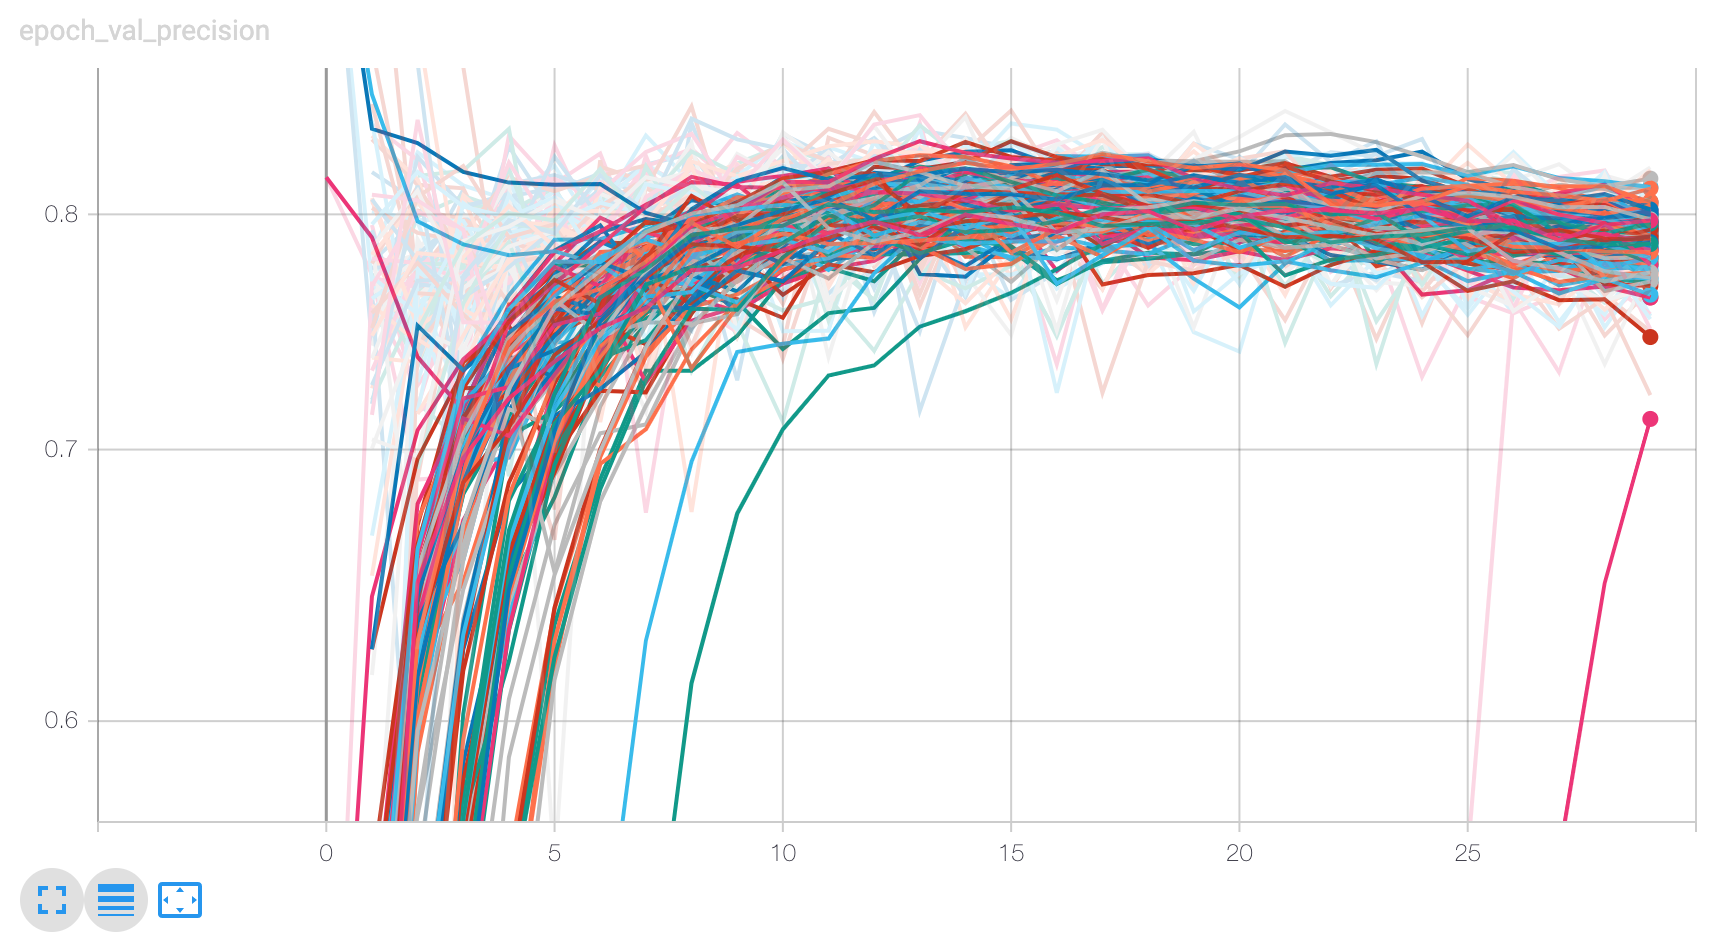
\includegraphics[width=0.89\linewidth]{figures/augmentation/val_precision.png}}
    \par\medskip
    \centering
    \subfloat[Recall]{\label{fig:augm_val_b}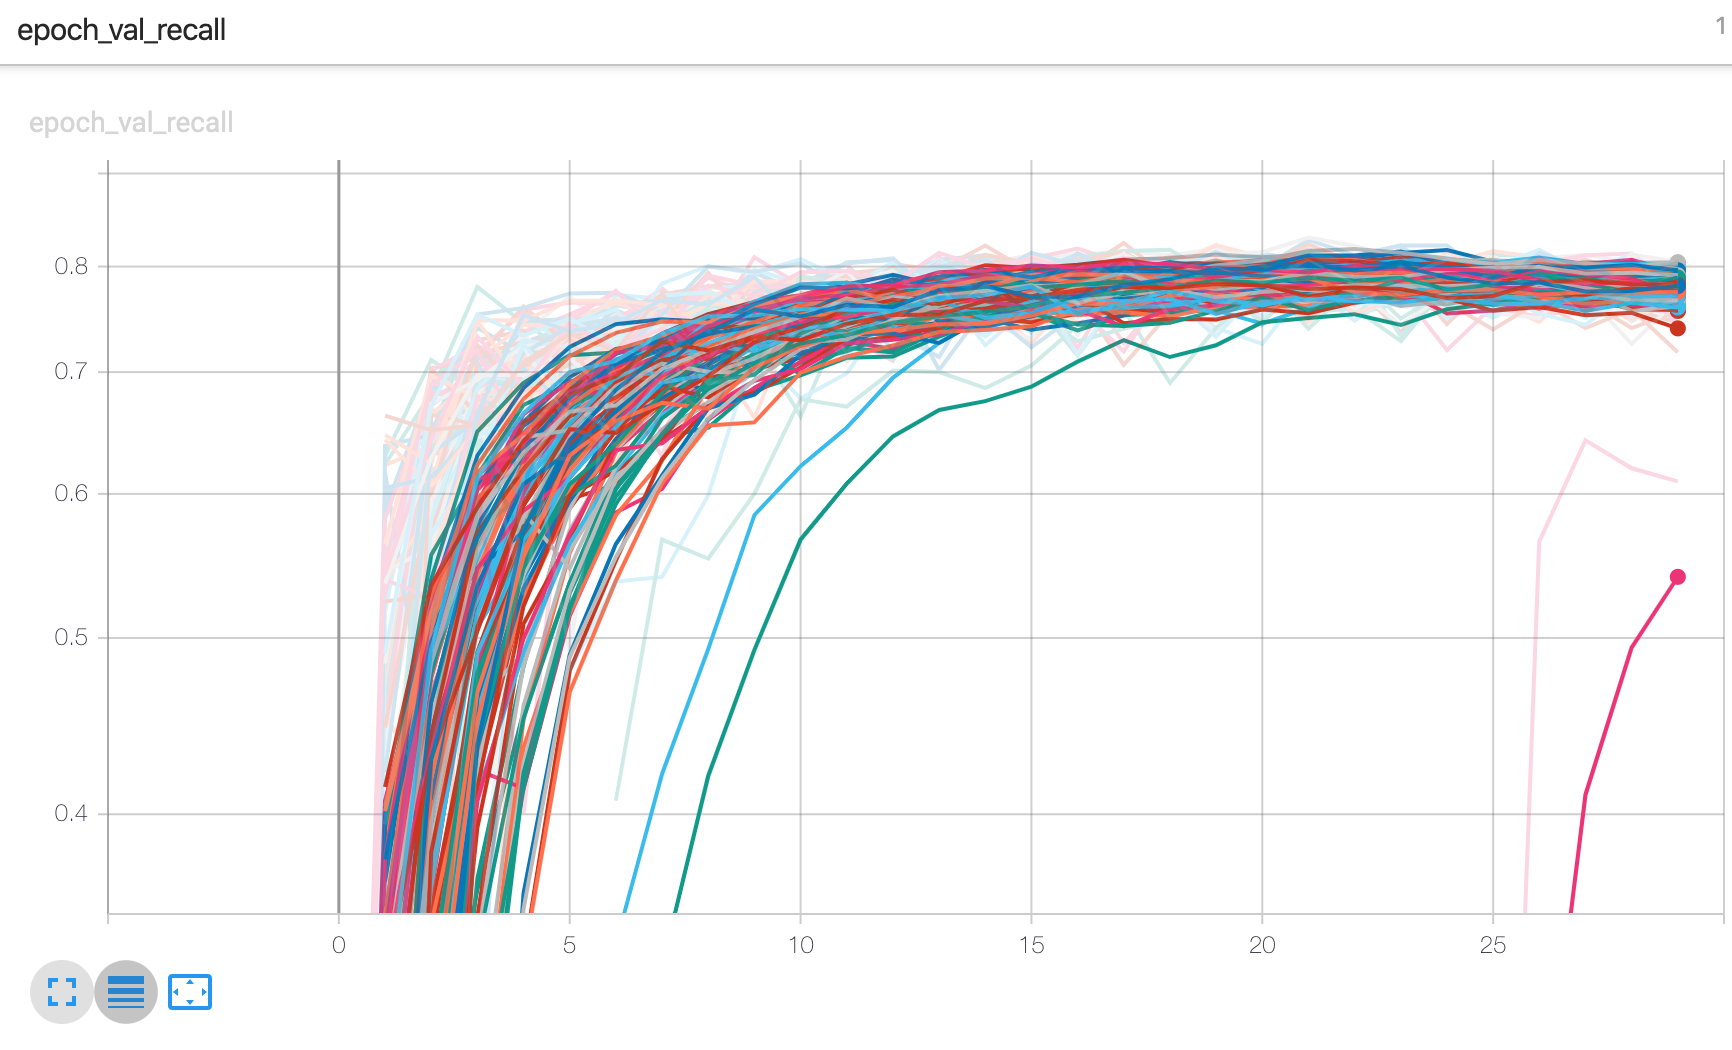
\includegraphics[width=0.89\linewidth]{figures/augmentation/val_recall.png}}
    \par\medskip
  \caption{Augmentation on Validation Set with 164 different combinations. The range of all results are close which indicates no clearly better combination(s) or method(s).}
  \label{fig:augm_val}
\end{figure}

\subsection{Results on Test Set}
Unfortunately, the scalar (graphs) can not be exported from TensorBoard for further analysis. We suspect this might be due to the resulting data size. Due to these limitation, or because these augmentation methods seem to not make a difference, each parameter is validated on the test individually with the "middle" value. E.g. width-shift was tested with a range of 0, 10 and 20. Therefore, the "middle" value for width-shift is 10. The only exception is vertical-flip since this is a Boolean value. This value is tested with 1 for true. The results are shown in the following table:

\begin{table}[h]
\centering
\begin{tabular}{ |p{3cm}|c|c|  }
 \hline
 \multicolumn{3}{|c|}{Augmentation results on test set} \\
 \hline
 Method & Precision & Recall\\
 \hline
 Baseline & 0.7019 & 0.7087\\
 Vertical-flip(1) & 0.6981 & 0.6891\\
 Rotation-range(10) & 0.6418 & 0.6346\\
 Zoom-range(10) & 0.7325 & 0.7196\\
 Height-shift(10) & 0.7047 & 0.6923\\
 Width-shift(10) & 0.6765 & 0.6635\\
 \hline
\end{tabular}
\end{table}

The vertical-flip and height-shift are close to the baseline results while the results for rotation-range and width-shift are lower. Only the results of zoom-range are higher than the baseline especially for the precision metric. However, it should be noted that these results likely have limited implication due to their ambiguity. No augmentation method seems to clearly outperform the baseline or clearly underperform. Rotation-range and width-shift seem to indicate worse performance but a confident conclusion that this indeed the case can not be made. Although zoom-range seem to perform better, the results are so close to the baseline that no confident conclusion can be drawn either. \\
It can be speculated that rotation of images does indeed lead to worse performance since an x-ray is more or less "straight" most of the times. This could lead to "irritating" patterns when the convolutional layers are generated. Theoretically, zoom-range would sustain the general pattern which may explain the seemingly better performance.








%% conclusion
\section* {Conclusion}

\begin{table}[h]
\centering
\begin{tabular}{ |p{4.5cm}|c|c|  }
 \hline
 \multicolumn{3}{|c|}{Results} \\
 \hline
 Method & Precision & Recall\\
 \hline
 Baseline & 0.7019 & 0.7087\\
 Undersampling & 0.6770 & 0.6651\\
 Oversampling & 0.3720 & 0.3702\\
 Augmentation vertical-flip(1) & 0.6981 & 0.6891\\
 Augmentation rotation-range(10) & 0.6418 & 0.6346\\
 Augmentation zoom-range(10) & 0.7325 & 0.7196\\
 Augmentation height-shift(10) & 0.7047 & 0.6923\\
 Augmentation width-shift(10) & 0.6765 & 0.6635\\
 \hline
\end{tabular}
\end{table}

The results are not meeting our expectations, regarding a distinct improvement of results due to dealing with class imbalance. No other method other than oversampling yielded in clear results from which a confident conclusion could be drawn. Oversampling likely lead to high overfitting which resulted in substantially lower scores in precision and recall which allow for the confident conclusion that oversampling leads to lower performance. The result of undersampling does not deviate substantially from the baseline. We suspect this is due to the fact that we made sure that the CNN does not overfit when trained with the initial, imbalanced, dataset. Since oversampling likely lead to overfitting, the first versions of our CNN did overfit on the initial, imbalanced, dataset as well for which we now suspect the class imbalance, undersampling maybe could have reduced overfitting by balancing the classes, if we did not specifically design our CNN to not overfit on the given, imbalanced, dataset. This opens the possibility for further research: "Would undersampling yield in different results if the CNN would initially overfit on the imbalanced dataset?". The results for the different data augmentation methods, also in combination with each other, were so close to the baseline that a conclusive implication is not possible. \\
To inspire further research, in-depth augmentation methods, like generating new images with generative adversarial networks (GAN), might be another approach. GANs extent from simple interpolation of images to actually learning from given instances to generate new ones.

%% acknowledgement
\section* {Acknowledgement}

\begin{table}[h]
\centering
\begin{tabular}{ |p{3cm}|c|  }
 \hline
 \multicolumn{2}{|c|}{Contribution} \\
 \hline
 \hline
 Name & Percentage\\
 \hline
 Pelinsu Çiftçioğlu & 5\%\\
 Lars Rass & 20\%\\
 Josef Dabrowski & 5\%\\
 Mark Limudjianto & 35\%\\
 Samuel Stroschein & 35\%\\
 \hline
\end{tabular}
\end{table}

Please take into consideration, that the current situation, due to the corona pandemic, had quite some impact on our project. \\
The early stages of the project, which included deciding on the topic, phrasing the research question and drafting the plan of attack, went as planned and everybody participated to their full extent. \\
However, the realisation of the project, which included research, coding, debugging and writing the report, was severely influenced by the current situation. \\
We insist to emphasize, that the contribution to the project in the table above are the result of an involuntary development. The non-EU exchange students in our team Pelinsu from Turkey and Josef from Australia understandably had more pressing matters to deal with under these highly dynamic circumstances. They constantly had to reevaluate measures taken by their home-countries and universities or even spontaneously organize a return flight.\\
Please take these circumstances into account, when evaluating this report. It would be highly appreciated.


%% The next two lines define the bibliography style to be used, and
%% the bibliography file.
%\bibliographystyle{ACM-Reference-Format}
\bibliographystyle{splncs04}
\bibliography{reference}

\end{document}